\subsection{Chapter 23 - The Theory of Special Relativity}

\subsubsection{Overview}\label{chap:specialrelativity}

In this chapter, we introduce the theory of Special Relativity, originally formulated by Albert Einstein in 1905. Along with the development of Quantum Mechanics, Special Relativity marks the start of ``modern physics'', and the introduction of theories to describe our world that are decidedly counter-intuitive.

\begin{framed}
\textbf{Learning Objectives}\\
\begin{itemize}
\item Understand the motivation for developing the Theory of Special Relativity.
\item Understand Einstein's postulates and their consequences.
\item Understand how to apply Einstein's postulates to describe simultaneity.
\item Understand how to model length contraction and time dilation.
\item Understand how to apply Lorentz transformations and make space-time diagrams.
\item Understand how to model the energy and momentum of a relativistic object.
\end{itemize}
\end{framed}

\begin{framed}
\textbf{Think About It}\\
Is it possible to time-travel into the future, so that you will be younger than people that are currently younger than you?

\begin{enumerate}
\item Yes, it's possible.
\item No, it is impossible because it would violate causality.
\item No, it is impossible because it's a ridiculous idea.
\end{enumerate}

\begin{framed}
\textbf{Answer}\\
\begin{enumerate}
\item
\end{enumerate}
\end{framed}
\end{framed}

\subsubsection{Introduction: The issue with Maxwell's equations}

% %%highlight the issue with Maxwell's equation
% %%%speed of ligth, Michelson and Morley

In Section~\ref{chapter:induction}, we summarized our knowledge of electromagnetism using Maxwell's four equations. As far as we can tell, this is the best description that we have of classical electric and magnetic phenomena (classical in the sense that the equations do not describe the behaviour of particles that are described by Quantum Mechanics). One of the consequences of Maxwell's equations is that they describe the existence of electromagnetic waves that propagate with a speed, $c$, given by:
\begin{equation}
c = \frac{1}{\sqrt{\epsilon_0\mu_0}}
\end{equation}
where $\epsilon_0$ and $\mu_0$ are the permittivity and permeability of free-space, respectively. We are familiar with waves that propagate through specific media. For example, ocean waves move through water and sound waves through air. The obvious question to ask about these electromagnetic waves is: ``In what medium do these waves propagate?''. In the late 1800s, it was thought that the Universe was bathed in a substance called the ``luminous ether'' (or just ``ether''), through which electromagnetic waves propagate. It was then thought that the speed, $c$, of these waves was, naturally, measured with respect to the ether. This led to the idea that there exists a special inertial frame of reference in the Universe, corresponding to that frame of reference in which light travels at a speed, $c$. This frame of reference would be at rest relative to the ether.

In the late 1880s, Michelson and Morley developed a clever experiment to measure the speed of the Earth relative to the ether. If the ether exists, and the Earth is moving through it, then a beam of light travelling parallel to the motion of the Earth should travel at a slightly different speed than a beam of light travelling in the perpendicular direction. However, Michelson and Morley conclusively demonstrated that this was not the case. There is no detectable motion of the Earth through a medium in which light (a electromagnetic wave) propagates. There is no ether. This was a very puzzling discovery, with strange implications for Maxwell's equations.

Let us demonstrate, through a simple example, an ``issue'' with the theory of electromagnetism. Rather, it is not an issue, but a very strange implication. Consider two infinitely-long wires, separated by a distance, $r$, each carrying a uniform charge per unit length, $\lambda$, as illustrated in Figure~\ref{fig:specialrelativity:twowire_electric}.

\begin{figure}[!htbp]
\centering
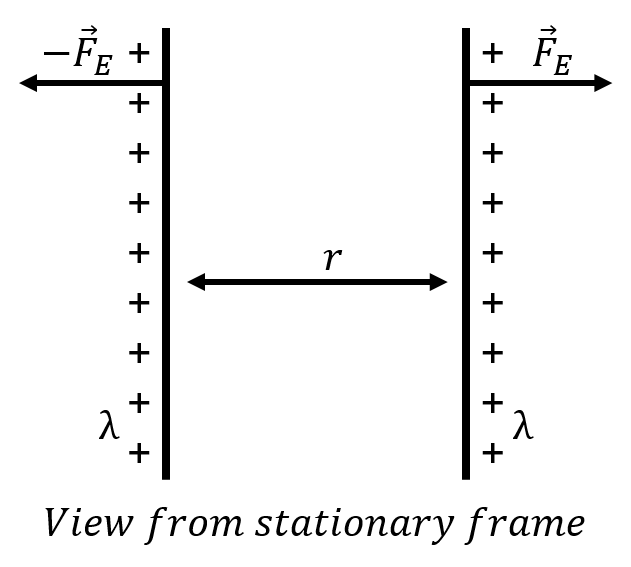
\includegraphics[width=0.4\linewidth]{files/twowire_electric-36eb50bad6978cca806e4c1857084eb6.png}
\caption[]{Two infinitely long charged wires exert a repulsive electric force on each other.}
\label{fig:specialrelativity:twowire_electric}
\end{figure}

We can easily calculate the magnitude of the repulsive electric force, $\vec F_E$, exerted by one charged wire on a section of length $l$ of the other wire. The magnitude of the electric field at a distance, $r$, from an infinitely-long wire with charge per unit length $\lambda$ is given by:
\begin{equation}
E = \frac{\lambda}{2\pi \epsilon_0r}
\end{equation}
A section of length $l$ of the other wire carries charge, $q=l\lambda$, so that the force on that section of wire has a magnitude:
\begin{equation}
F_E=qE=\lambda l \left( \frac{\lambda}{2\pi \epsilon_0r}\right) = \frac{\lambda^2 l}{2\pi \epsilon_0r}
\end{equation}
And the force per unit length, on either one of the wires, has a magnitude:
\begin{equation}
\frac{F_E}{l}=\frac{\lambda^2}{2\pi \epsilon_0r}
\end{equation}
This is the only force exerted on one of the wires, and will thus allow us to completely specify the motion of that wire (we know all of the forces exerted on the wire, so we can use Newton's Second Law to determine its acceleration and describe its motion).

Consider the same two wires, each carrying a charge per unit length, as viewed from a frame of reference that is moving downwards (parallel to the wires), with a speed, $v$. In this frame of reference, the infinite wires still have a net charge per unit length, but they also appear to have an upwards moving current, $I$, since we observe positive charges moving upwards through space.

\begin{figure}[!htbp]
\centering
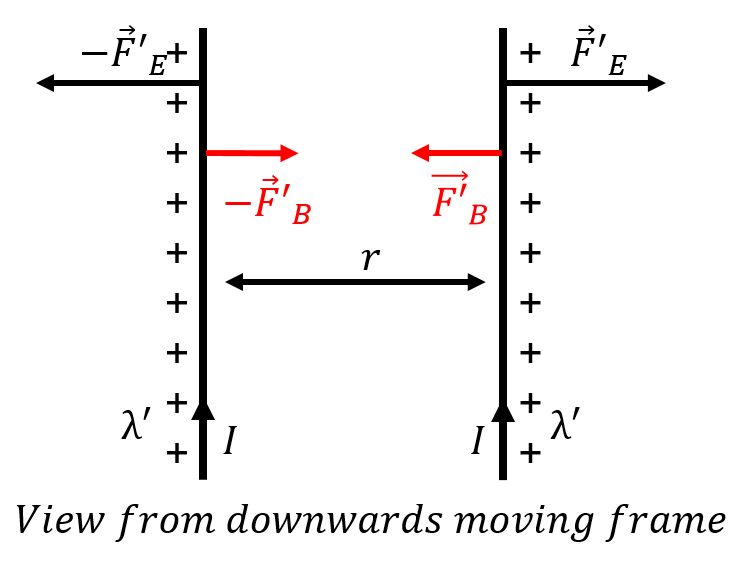
\includegraphics[width=0.4\linewidth]{files/twowire_magnetic-535a8de6057d101e2e69bb7bd86ee6ae.png}
\caption[]{Two infinitely-long charged wires as viewed from a down-going frame of reference will appear to have upwards-going currents that will result in an attractive magnetic force between the wires.}
\label{fig:specialrelativity:twowire_magnetic}
\end{figure}

In this new frame of reference, we see two wires with charges on them, moving upwards with speed, $v$. In an interval of time, $\Delta t$, we see a length of wire, $\Delta x=v\Delta t$, go by, with total charge, $\Delta Q=\lambda' \Delta x$. For reasons that will be clear below, we use a different charge density, $\lambda'$, in the moving frame of reference, although we \textit{expect} that $\lambda'=\lambda$. This corresponds to a current, $I$, given by:
\begin{equation}
I=\frac{\Delta Q}{\Delta t}=\lambda'\frac{\Delta x}{\Delta t}=\lambda' v
\end{equation}
Thus, in the downward going frame of reference, we see two wires with upwards current in them, and these wires must extract an attractive magnetic force between each other, with magnitude (per unit length):
\begin{equation}
\frac{F'_B}{l} = -\frac{\mu_0 I_1I_2}{2\pi r}=-\frac{\mu_0 I^2}{2\pi r}=-\frac{\mu_0 \lambda'^2 v^2}{2\pi r}
\end{equation}
where the prime (') on the force indicates that the force is measured in this different inertial frame of reference, and the minus sign indicates that it is in the opposite direction from the repulsive electric force.

In the downwards going frame of reference, the wires are still charged, and must still exert a repulsive electric force, with magnitude (per unit length):
\begin{equation}
\frac{F'_E}{l}=\frac{\lambda'^2}{2\pi \epsilon_0r}
\end{equation}
where, again, we used primes ('), to denote quantities that are measured in the moving frame of reference.

The description of how the wires will move should not depend on the frame of reference in which we choose to model the wires (they will move under the forces exerted on them regardless of whether we are observing them from a fixed or a moving point, and indeed regardless of whether we observe them at all!). Thus, the net force (per unit length) exerted on a wire cannot depend on our frame of reference. The total repulsive electric force, $F_E$, calculated in the stationary frame of reference must be equal to the sum of the magnetic and electric forces, $F'_B$ and $F'_E$, calculated in the moving frame of reference \footnote{This statement is generally true for Special Relativity, because the force is exerted in the direction perpendicular to that of motion.}:
\begin{equation}
\frac{F_E}{l}&=\frac{F'_E}{l}+\frac{F'_B}{l}\\
\frac{\lambda^2}{2\pi \epsilon_0r}&=\frac{\lambda'^2}{2\pi \epsilon_0r}  -\frac{\mu_0 \lambda'^2 v^2}{2\pi r}
\end{equation}
where we recognized that the charge per unit length, $\lambda'$, must be different in the moving frame of reference, or the above would give an inconsistent equation (the electric forces would cancel and we would find that the magnetic force is equal to zero). Thus, the repulsive electric force must be larger as observed in the moving frame of reference, or the net force on the wire would be different when evaluated in the two frames of reference. This is a truly bizarre conclusion, as we will see.

Before proceeding, let us clearly state our assumptions in modelling the force between the two charged wires:

\begin{enumerate}
\item The net force on the wire, allowing us to describe its motion, cannot depend on our frame of reference. We expect the laws of physics to be applicable from any inertial frame of reference.
\item We assume that Maxwell's equations hold in all inertial frames of reference. In particular, we assume that the constants, $\mu_0$ and $\epsilon_0$, are the same in all inertial reference frames.
\end{enumerate}

The first assumption allows us to state that the net force in the two frames of reference must be the same. The second assumption implies that we must change the charge density, $\lambda'$, in the moving frame of reference, since the constants must remain the same, and this is the only quantity that can lead to a different electric force in the moving frame of reference (which is required if the net force is to be the same, according to our first assumption). Let us determine the new charge density, $\lambda'$, in terms of the charge density that is measured at rest. Starting with the requirement that the net force on the wire must not depend on the frame of reference, we find:
\begin{equation}
\frac{\lambda^2}{2\pi \epsilon_0r}&=\frac{\lambda'^2}{2\pi \epsilon_0r}  -\frac{\mu_0 \lambda'^2 v^2}{2\pi r}\\
\lambda^2&=\lambda'^2-\epsilon_0\mu_0\lambda'^2 v^2\\
\lambda^2&=\lambda'^2(1-\epsilon_0\mu_0v^2)\\
\therefore \lambda'&=\lambda \frac{1}{\sqrt{\epsilon_0\mu_0-v^2}}
\end{equation}
Finally, recognizing that we can use the speed of light, $c$, to replace the combination of constants, $\epsilon_0\mu_0$, we find:
\begin{equation}
\lambda'&=\lambda \frac{1}{\sqrt{1-\frac{v^2}{c^2}}}
\end{equation}
Thus, the charge per unit length on the wire is larger when measured from the moving frame of reference ($\lambda'$ is greater than $\lambda$ if $v<c$). It should be somewhat bothersome to you that the charge per unit length depends on the frame of reference in which it is measured, but this is the only way for our two assumptions to hold.

So far, this has just been some math to ensure that ``things work out'', namely that our description of the motion of the wire does not depend on our frame of reference. However, the consequences of what we just derived are profound. We concluded that the charge per unit length on a wire depends on our frame of reference.

Since we are dealing with infinitely long wires, we can draw two lines to define a section of the wire in the rest frame, as in Figure~\ref{fig:specialrelativity:twowire_chargedensity}. The charge per unit length on the wire, $\lambda$, is found by counting the number of charges between the two lines and dividing that by the distance between the two lines. Now, both an observer at rest relative to the wire, and one that is moving relative to the wire will agree on the number of charges contained between the two lines. They will both count the same number. Thus, if the observer moving relative to the wire is to measure a larger charge density, then the distance between the lines must be smaller for that observer! To the observer moving relative to the wire, the wire is actually shorter. It does not appear to be shorter, it IS shorter!

\begin{figure}[!htbp]
\centering
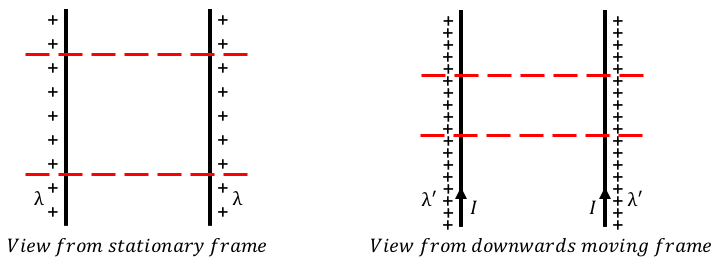
\includegraphics[width=0.8\linewidth]{files/twowire_chargedensit-b5a881d42989d15971cd5cefb0e170e2.png}
\caption[]{Two infinitely-long charged wires as viewed from a rest frame and a moving frame. In order for the charge density to be greater in the moving reference frame, the wire must be shorter. For an infinitely long wire, this is depicted by showing that if we use two lines (red dashed lines) to define a section of wire in the rest frame, those lines will be closer together in the moving frame.}
\label{fig:specialrelativity:twowire_chargedensity}
\end{figure}

To summarize, by requiring that the laws of physics are the same in all inertial frames of reference, and by requiring that Maxwell's equations are the same in all inertial frames of reference, we conclude that the charge per unit length that is measured on a wire must depend on the frame of reference in which it is measured. Since it cannot be the number of charges on the wire that depends on the frame of reference, it must be the length of the wire that depends on the frame of reference. Thus, either we accept that Maxwell's equations are incorrect, or we accept that they are correct but that they imply that objects shrink in length when they are moving (regardless of whether charges are involved). It turns out that the latter choice provides a better description of nature (and one that has not been invalidated!).

An additional consequence of accepting these implications from Maxwell's equations is that the definition of the electric and magnetic fields must depend on the frame of reference. In the example from this section, we saw that what looks like an electric field in the stationary frame of reference can appear as the combination of a magnetic and electric fields in a moving frame of reference.

\subsubsection{Einstein's postulates}

% Two postulates
% Simulataneity

Albert Einstein was the first to provide a complete description of how to deal with the issues that arise from Maxwell's equations when these are examined in different inertial frames of reference. The Theory of Special Relativity is based on Einstein's two postulates:

\begin{enumerate}
\item The laws of physics are the same in all inertial reference frames. There is no experiment that can be performed to determine whether one is at rest or moving with constant velocity.
\item The speed of light propagating in vacuum is the same in all inertial reference frames. Any observer in an inertial frame of reference, regardless of their velocity, will measure that light has a speed of $c$ when it propagates in vacuum.
\end{enumerate}

These postulates are equivalent to the assumptions that we made above to model the force between the two wires (we stated that the constants, $\epsilon_0$ and $\mu_0$, were independent of the reference frame, instead of $c$). While the first postulate is perhaps ``acceptable'' to our common sense, the second one grossly defies common intuition. Consider two archers, as illustrated in Figure~\ref{fig:specialrelativity:arrow}.

\begin{figure}[!htbp]
\centering
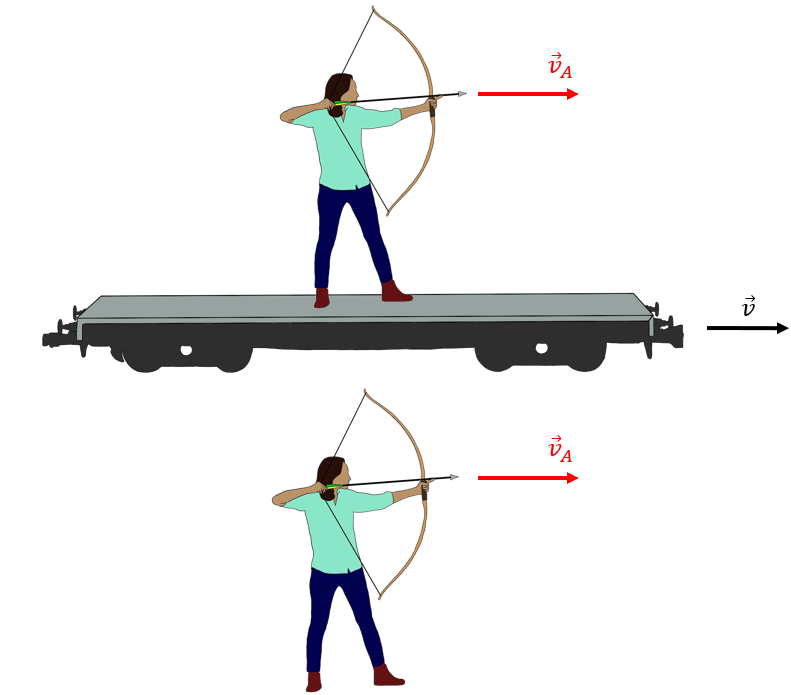
\includegraphics[width=0.5\linewidth]{files/arrow-e43be0a8321345241200b467b38d2883.png}
\caption[]{Two archers can fire an arrow with speed $v_A$. As measured in the frame of reference of the ground (of the target), the arrow fired from the archer that is on the train will have a higher speed.}
\label{fig:specialrelativity:arrow}
\end{figure}

Both archers can fire an arrow with speed $v_A$. One archer fires her arrow from the ground, and that arrow will hit its target with speed $v_A$. The other archer is on a train that is moving with speed $v$ in the same direction that she wishes to shoot her arrow. She measures her arrow to leave her bow with speed $v_A$, but, as seen from the ground (and from the target), her arrow has a speed $v_A+v$, and it will hit the target with a higher speed, as expected.

Now, consider two people that instead fire a pulse of laser light at a target on the ground, as illustrated in Figure~\ref{fig:specialrelativity:laser}.

\begin{figure}[!htbp]
\centering
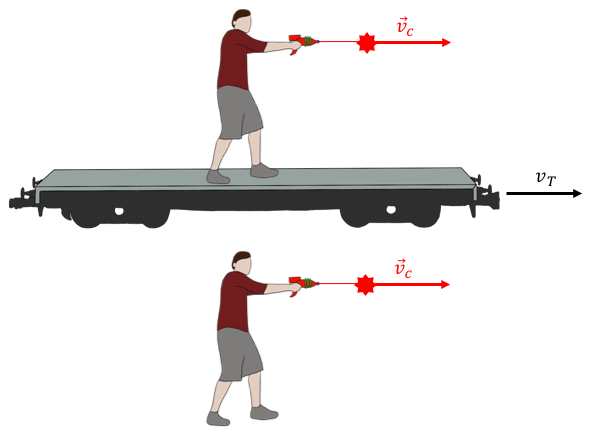
\includegraphics[width=0.5\linewidth]{files/laser-5fee8c8b50f80a779a31bd60586c2636.png}
\caption[]{Two people fire a laser pulse. Regardless of whether the pulse of laser light was fired from a moving train or from the ground, it will have a speed of $c$ in all frames of reference.}
\label{fig:specialrelativity:laser}
\end{figure}

In this case, according to Einstein's second postulate, the speed of the pulses as measured on the ground (by the target), will be $c$, regardless of whether one of the pulses was fired from a moving train. This is truly strange and not compatible with our experience. For example, imagine that the train moves close to the speed of light. The person on the train would fire a laser pulse that he would observe to move away from him at the speed of light. However, when observed from the ground, we would see the pulse of light move away from them very slowly.

\paragraph{Simultaneity}

As a first consequence of Einstein's postulates, let us consider the notion of simultaneity. Figure~\ref{fig:specialrelativity:platform_rest} shows Alice on the platform of a train station. Alice is midway between two clocks, $A$ and $B$. Both identical clocks were configured so that they send a pulse of laser light when the time is 20 minutes past four o'clock. Since Alice is midway between the clocks, if they emit their pulses of light at the same time, then Alice will see two pulses of light arrive at her location at the same time. She signals that the two pulses of light have reached her at the same time by raising her hands.

\begin{figure}[!htbp]
\centering
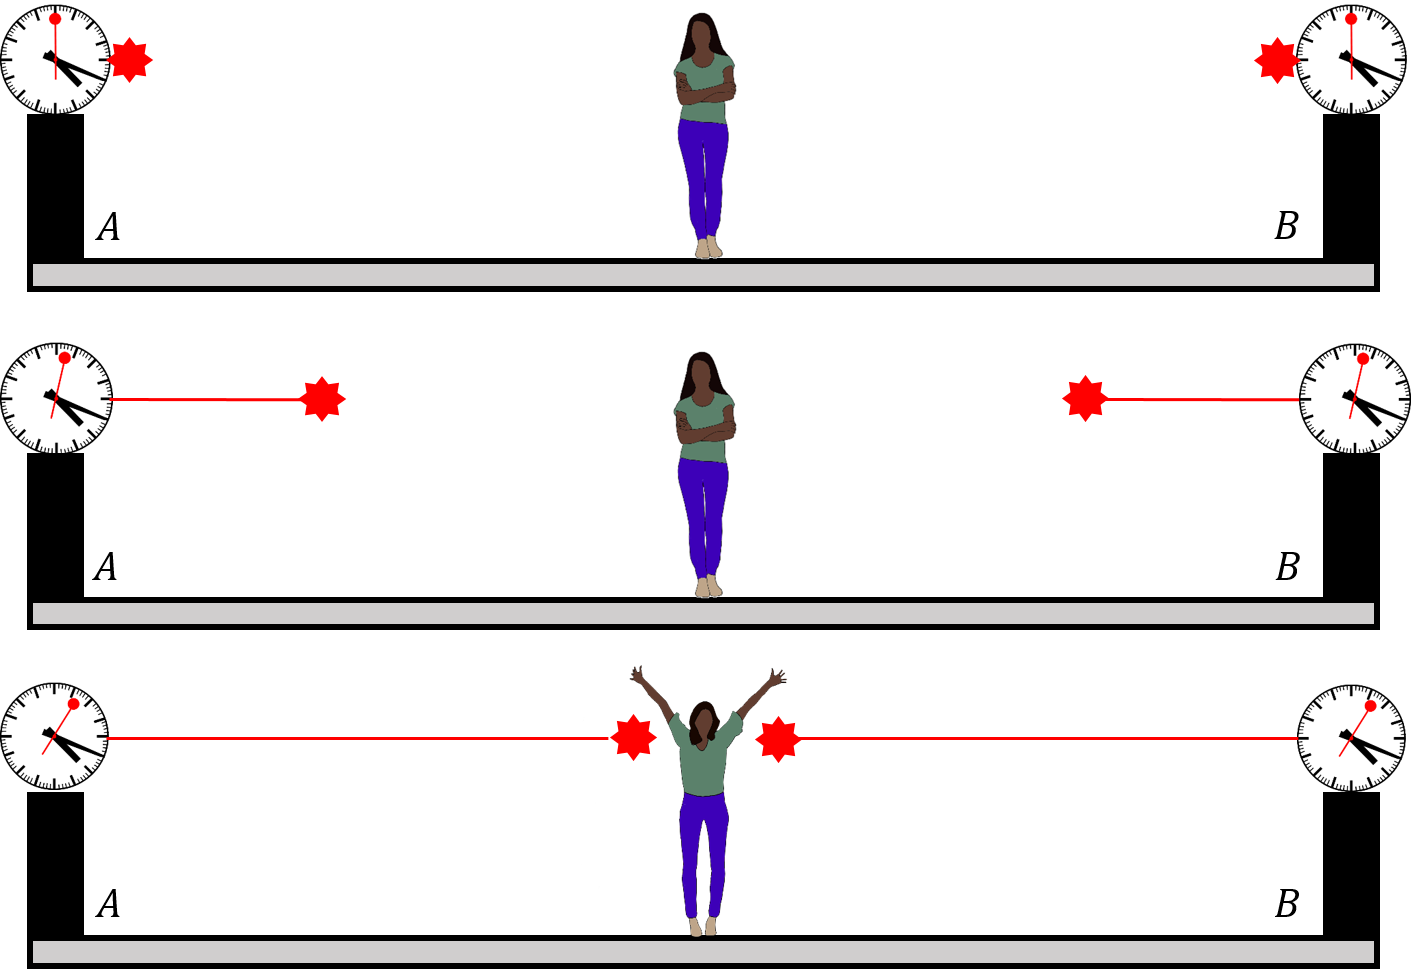
\includegraphics[width=0.7\linewidth]{files/platform_rest-b420067c83cb3647a868c3bff6795c0d.png}
\caption[]{Alice is equidistant from two clocks. The clocks fire a laser pulse when the time is 20 past four, and Alice observes both pulses arriving at her location at the same time, concluding that the pulses were emitted by the clocks at the same time.}
\label{fig:specialrelativity:platform_rest}
\end{figure}

Brice is located on a train that is travelling with speed, $v$, in the direction from clock $A$ to clock $B$, as illustrated in Figure~\ref{fig:specialrelativity:platform_moving}. He sees Alice and the platform moving towards him.

\begin{figure}[!htbp]
\centering
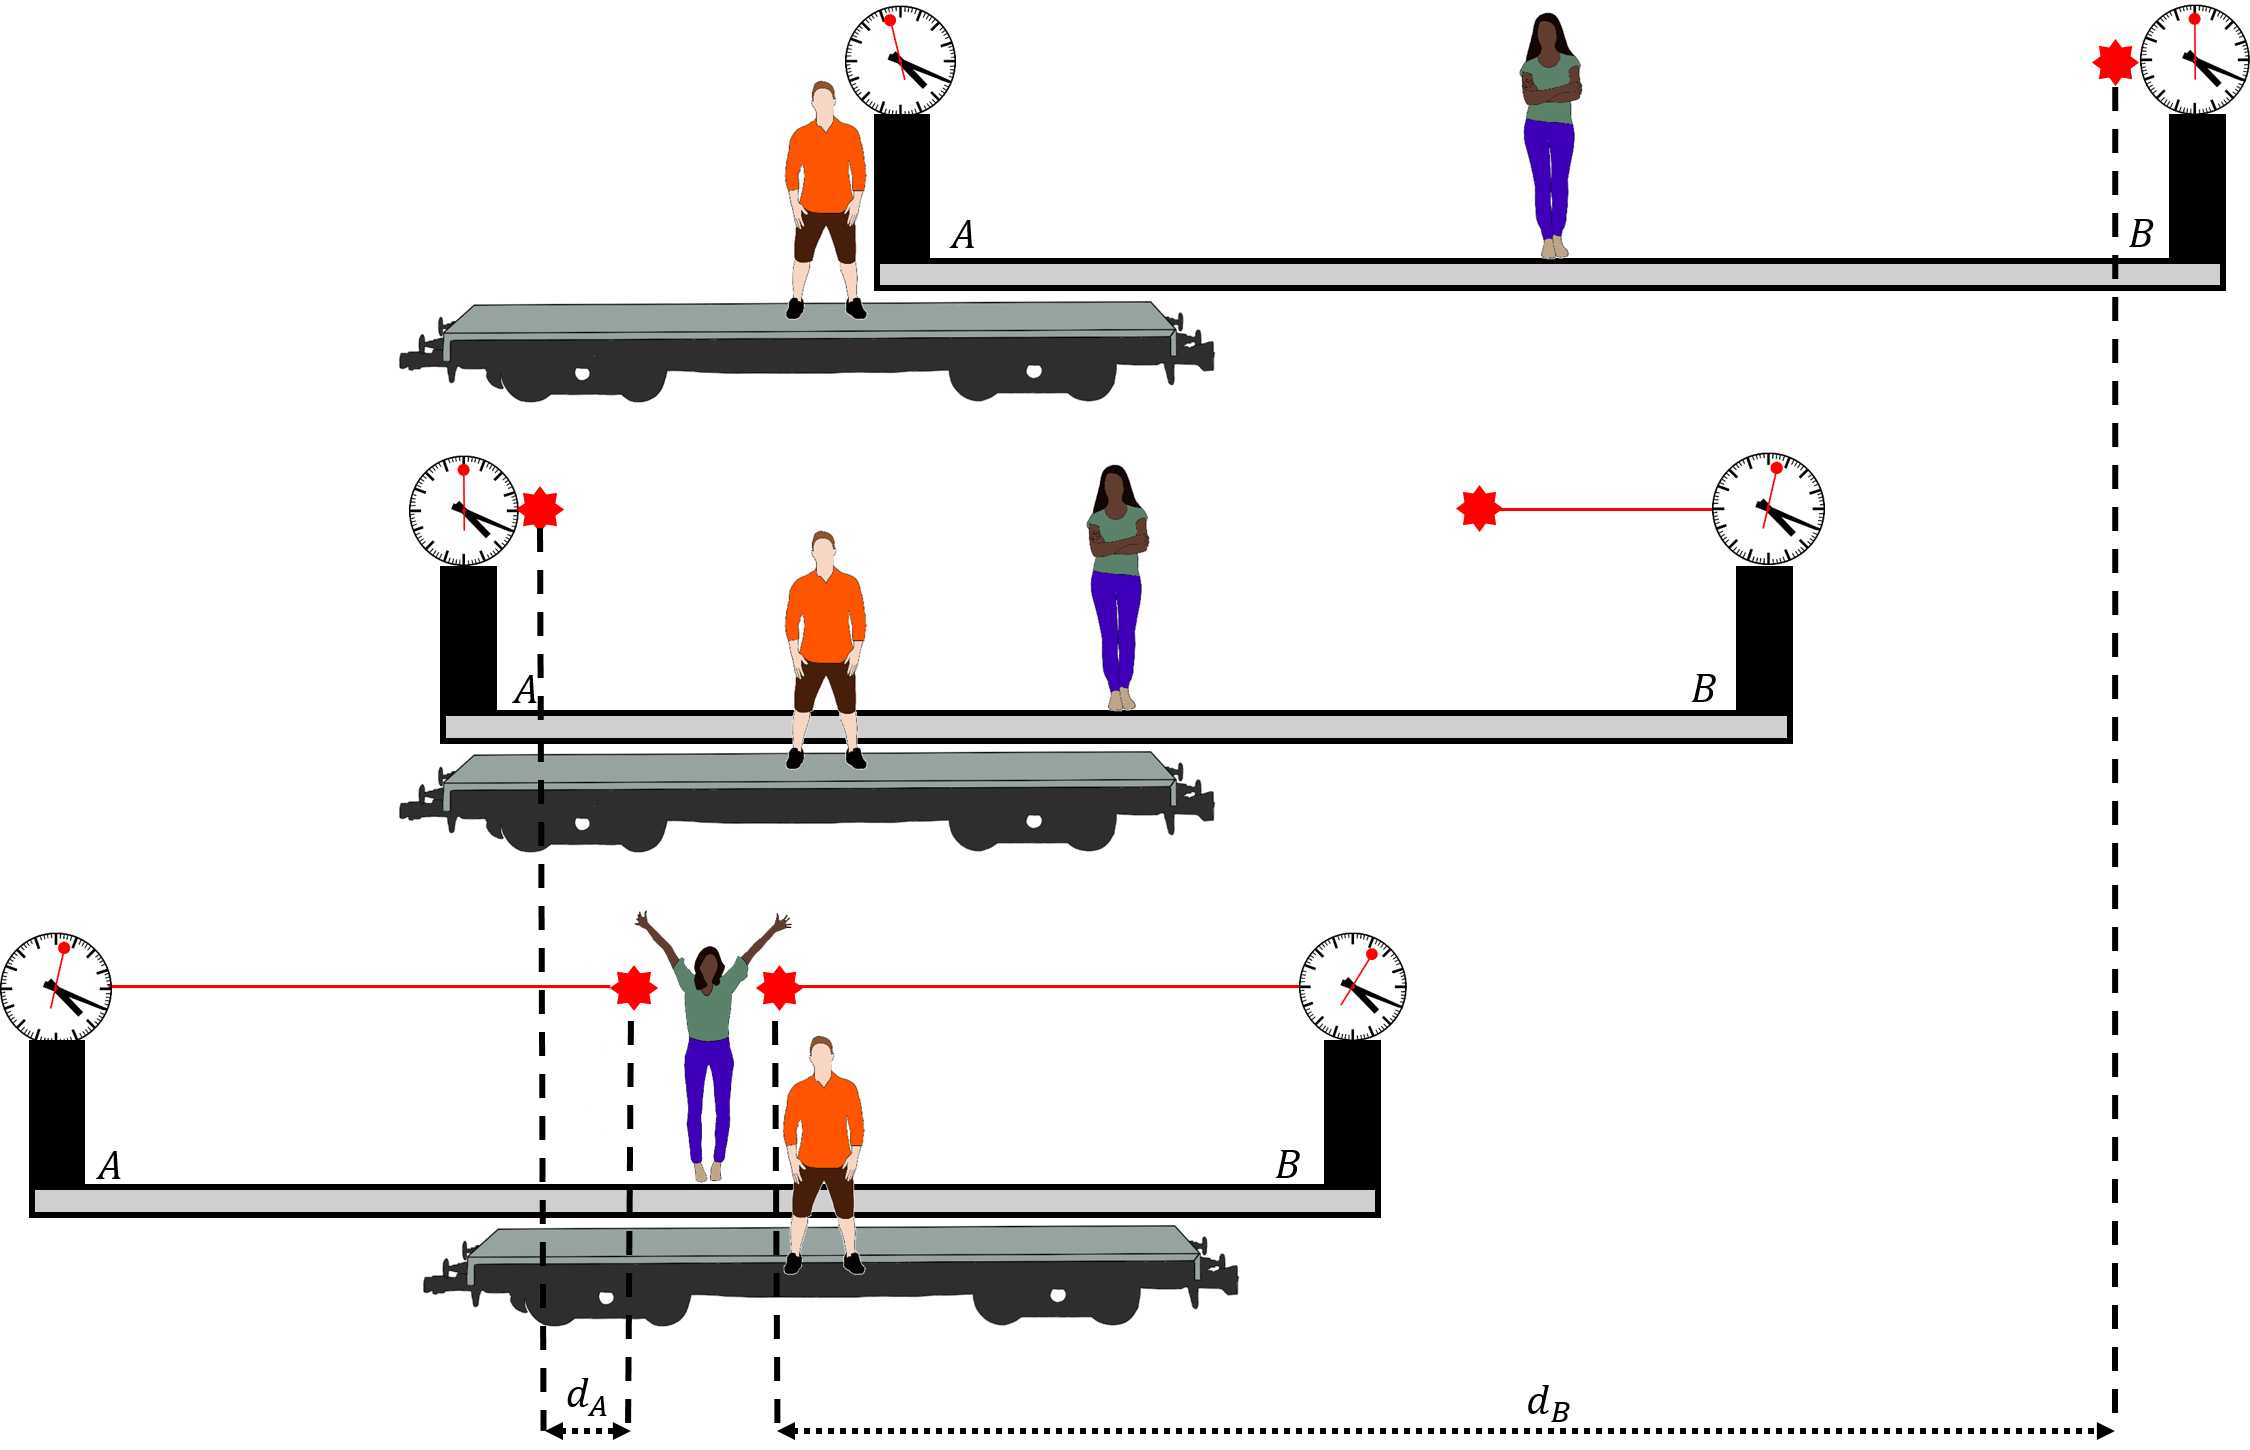
\includegraphics[width=0.8\linewidth]{files/platform_moving-73adb17069939401ece5c1c52eb63fba.png}
\caption[]{Brice is on a moving train, and, from his perspective, it is Alice and the platform that are moving towards him. Brice must conclude that the pulse from clock $B$ was emitted earlier, since it must travel further than the pulse emitted from clock $A$ to reach Alice at the same time.}
\label{fig:specialrelativity:platform_moving}
\end{figure}

Brice must agree that the two pulses arrived at Alice's location at the same time, since he can also see her raise her hands. In Brice's frame of reference, the two pulses of light must travel with the speed of light (Einstein's second postulate). Once the pulse of light has been emitted from clock $B$, Brice observes that Alice is moving away from the location of where the pulse was emitted, so that pulse must travel a large distance, $d_B$. On the other hand, once the pulse from clock $A$ is emitted, Brice observes that Alice moves towards where the pulse was emitted, so it only needs to travel a shorter distance, $d_A$, in order to reach Alice. Thus, for both pulses to arrive at Alice at the same time and travel at the speed of light, the pulse from clock $B$ had to be emitted first, according to Brice.

That is, while Alice measures the clocks to be synchronized and emit pulses at the same time, Brice measures that clock $B$ is running ahead of clock $A$. The two observers, Alice and Brice, in different reference frames, cannot agree on whether two events are simultaneous. Even worse, if a third observer, {\textbackslash}chloens, is located on a train going in the opposite direction from Brice's train, she will conclude that the pulse from clock $A$ was emitted earlier than the pulse from clock $B$. A consequence of Einstein's postulates is that observers in different frames of reference will not agree on whether two events happen at the same time, and in some cases, as the one we illustrated, the observers will not agree on which event happened first. Think of the implications for causality!

\subsubsection{Time dilation}

Einstein was famous for his ``thought experiments'', which allow us to understand the consequences of a theory by performing thought experiments that would be impractical to actually carry out (such as the experiment with Alice and Brice described above, which would be impractical to carry out, since the speed of light is so high that Brice would never notice that clock $A$ emitted the pulse slightly earlier).

Imagine that we build a clock using a pulse of light travelling (oscillating) back and forth between two mirrors, separated by a distance, $L$, as illustrated in Figure~\ref{fig:specialrelativity:clock_rest}.

\begin{figure}[!htbp]
\centering
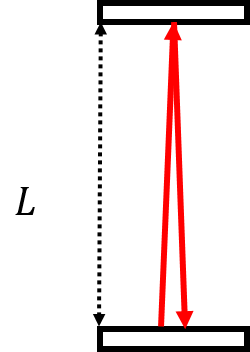
\includegraphics[width=0.2\linewidth]{files/clock_rest-2b24dfaa579d2edf2fef42f2f97bf7d5.png}
\caption[]{A clock is made by having a pulse of light bounce back and forth between two parallel mirrors separated by a distance, $L$.}
\label{fig:specialrelativity:clock_rest}
\end{figure}

Since the speed of light is $c$, the time that it will take for the pulse of light to travel back and forth between the two mirrors, namely the period of the clock, is given by:
\begin{equation}
\Delta t = \frac{2L}{c}
\end{equation}
where the speed of light, $c$, is given by the total distance travelled by the pulse of light divided by the time taken to do so:
\begin{equation}
c=\frac{2L}{\Delta t}
\end{equation}
Now, imagine placing this clock on a spaceship that travels with speed $v$, perpendicular to the direction of the movement of the light. The clock is illustrated in Figure~\ref{fig:specialrelativity:clock_moving}, as seen from the ground.

\begin{figure}[!htbp]
\centering
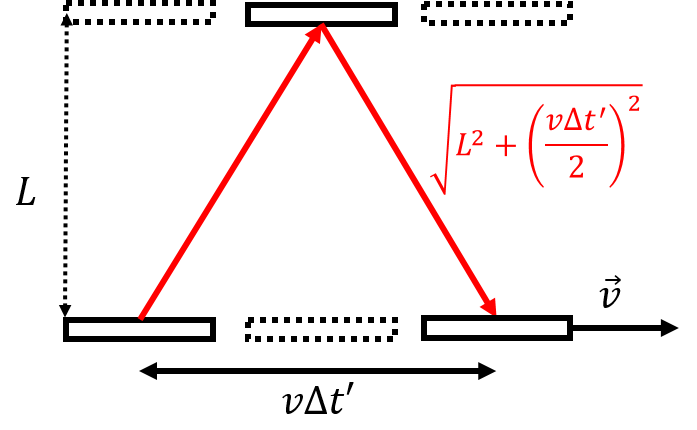
\includegraphics[width=0.5\linewidth]{files/clock_moving-bec37f43069648c48ba9eceb8c95a68f.png}
\caption[]{A clock is made by having a pulse of light bounce back and forth between two parallel mirrors separated by a distance, $L$. When the clock is placed on a spaceship moving with speed, $v$, the light travels a longer distance before completing a full cycle, as observed by someone not travelling with the clock.}
\label{fig:specialrelativity:clock_moving}
\end{figure}

From the perspective of a person watching the clock go by, the pulse of light travels a larger distance over one clock period, since the mirrors move to the right as the pulse of light moves up and down. However, by Einstein's second postulate, the pulse of light must still travel with the same speed, $c$, so it must take the pulse of light longer to bounce between the two mirrors than it did when the clock is at rest. Let us determine the relationship between the period of the clock, $\Delta t$, measured when the clock is at rest, and the period of the clock, $\Delta t'$, as measured by an observer that sees the clock go by with speed, $v$.

To an observer that sees the clock move by with speed, $v$, the speed of the pulse of light, which must also be equal to $c$, is given by:
\begin{equation}
c&=\frac{2\sqrt{L^2+\left(\frac{v\Delta t'}{2}\right)^2}}{\Delta t'}
\end{equation}
where the distance in the numerator was simply found by Pythagoras' theorem, as the spaceship will travel a horizontal distance, $v\Delta t'$, as measured by the observer that is not moving with the spaceship. Squaring this relationship, we can isolate the period of the clock, $\Delta t'$, as measured by the observer that sees the clock move with speed, $v$:
\begin{equation}
c^2&=\frac{4L^2}{\Delta t'^2}+v^2\\
\Delta t'^2 (c^2-v^2)&=4L^2\\
\therefore \Delta t' &= 2L\frac{1}{\sqrt{c^2-v^2}}\\
&=\frac{2L}{c}\frac{1}{\sqrt{1-\frac{v^2}{c^2}}}
\end{equation}
Note that the term $2L/c$ is simply the period of the clock as measured in a frame of reference where the clock is stationary. Thus, we can relate the two clock periods:
\begin{equation}
\boxed{\Delta t' = \Delta t \frac{1}{\sqrt{1-\frac{v^2}{c^2}}}}
\end{equation}
To re-iterate: the period of the clock, $\Delta t'$, as measured in a frame of reference that is moving relative to the clock is longer than the period of the clock, $\Delta t$, as measured in the ``rest frame'' of the clock (the reference frame where the clock is stationary). We call this effect \textbf{``time dilation''}, and it is not just some mathematical curiosity. The clock that we imagined with a pulse of light is a real clock that one could actually construct; we could use it to measure time. That clock will appear to tick slower if it is moving. \textbf{Time goes by slower in a moving reference frame}. If a person climbs on a ship that is moving, that person will age at a slower rate than a person that remained on Earth. By travelling at high speeds, you effectively travel into the future, as observed on Earth. The equation above allows us to relate the amount of time that went by in one reference frame to the amount of time that went by in a different frame of reference.

We define the time that is measured at rest as the ``proper time''. In our example, $\Delta t$ is the proper time (proper period) for the clock, since it is defined in a frame of reference where the clock is at rest. The ``dilated time'', $\Delta t'$, is measured in a frame of reference that is moving relative to the clock.

The factor by which time is dilated comes up often in Special Relativity, and is called the gamma factor:
\begin{equation}
\boxed{\gamma = \frac{1}{\sqrt{1-\frac{v^2}{c^2}}}}
\end{equation}
As a corollary to Einstein's postulates, we will see that nothing can ever exceed the speed of light in vacuum. The gamma factor is always greater than one, since $v$ (the speed between the two different inertial frames of reference) must always be smaller than $c$. You may also recognize that the gamma factor appeared in our introductory example with the force between two wires. Here, we derived the gamma factor from kinematic considerations, whereas in the example with the two wires, it came straight out of the equations for electromagnetism.

\begin{framed}
\textbf{Checkpoint}\\
What is gamma for a speed of $v=0.75c$?

\begin{enumerate}
\item 1.51
\item 0.75
\item 75
\item 1.68
\end{enumerate}

\begin{framed}
\textbf{Answer}\\
\begin{enumerate}
\item
\end{enumerate}
\end{framed}
\end{framed}

\begin{framed}
\textbf{Checkpoint}\\
What speed, $v$, corresponds to a gamma factor of 2.5?

\begin{enumerate}
\item $v=2.5c$
\item $v=0.92c$
\item $v=0.25c$
\item $v=0.47c$
\end{enumerate}

\begin{framed}
\textbf{Answer}\\
\begin{enumerate}[resume]
\item
\end{enumerate}
\end{framed}
\end{framed}

Time-dilation is a real effect that has been observed, for example, by placing high precision atomic clocks on an airplane to observe their period slow down. Another example of time-dilation is the fact that we observe many particles called muons at the surface of the Earth. Muons are very similar to electrons, except that they have a larger mass, and that they are unstable (they radioactively decay into an electron and neutrinos, after $2.2 {\rm \mu s}$ on average). Muons are produced in large amounts when cosmic rays (high energy particles from outside our Solar System) strike the molecules in our upper atmosphere, at altitudes of tens of kilometres. As the muons travel down towards the Earth, they decay.

Suppose that muons are produced travelling at the speed of light; in that case, they would travel a distance $d=(3\times 10^{8} {\rm m/s})(2.2\times 10^{ -6} {\rm s})=660 {\rm m}$, on average, before decaying. However, muons are produced tens of kilometres above the surface of the Earth, travel slower than the speed of light, and yet, we are able to detect many muons at the surface of the Earth. We would expect that all muons would have decayed before reaching the surface of the Earth.

We can understand this in terms of time dilation; in the reference frame of the muon, the muon decays after $\Delta t=2.2 {\rm \mu s}$. In a reference frame from which the muon appears to move with speed $v$, the ``clock'' that measures how long the muon has existed ticks slower. Thus, from the Earth, we observe that the muon takes longer than $2.2 {\rm \mu s}$ to decay, giving it time to reach the surface of the Earth.

\begin{framed}
\textbf{Example 23.1}\\
A muon travels with a speed of $0.9c$ as observed from the surface of the Earth. As measured in the frame of reference of the Earth, how far has the muon travelled after $2.2 {\rm \mu s}$ have elapsed \textbf{in the muon's frame of reference}?

\begin{framed}
\textbf{Solution}\\
The muon is travelling with a speed of $v=0.9c$ relative to the Earth, thus the gamma factor is given by:
\begin{equation}
\gamma = \frac{1}{\sqrt{1-\frac{v^2}{c^2}}} =\frac{1}{\sqrt{1-0.9^2}}=2.29
\end{equation}
The amount of time that goes by in the frame of reference of the Earth, $\Delta t$, when $\Delta t'=2.2 {\rm \mu s}$ has gone by in the muon's frame of reference will be dilated by the gamma factor. $\Delta t'$ is the proper time in the muon frame's of reference, which corresponds to a longer time in Earth's frame of reference:
\begin{equation}
\Delta t = \gamma \Delta t' = (2.29)(2.2 {\rm \mu s})=5.0 {\rm \mu s}
\end{equation}
In the frame of reference of the Earth, the muon has travelled a distance:
\begin{equation}
d' = v\Delta t'=(0.8c)(5.0 {\rm \mu s})=1350 {\rm m}
\end{equation}
\textbf{Discussion:} In this example, we see that an object, such as a muon, that travels with at 90 percent of the speed of light will have a gamma factor around 2. Thus, from the Earth's frame of reference, it appears that the muon ``ages'' at about half of the rate at which one would observe the muon to age if moving along with the muon. This is the mechanism that allows muons to exist much longer than $2.2 {\rm \mu s}$ when they are travelling relative to the Earth.

Also, in Earth's reference frame, the muon travels a distance of $1350 {\rm m}$ in the period of time between being produced and decaying. In the reference frame of the muon, only $2.2 {\rm \mu s}$ elapse as the Earth moves closer to the muon, at the same speed. In the reference frame of the muon, the Earth has travelled a distance:
\begin{equation}
d' = v\Delta t=(0.9c)(2.2 {\rm \mu s})=594 {\rm m}
\end{equation}
Thus, as viewed from the muon's frame of reference, the distance that it travelled between being produced and decaying is about half the distance as measured in the Earth's reference frame. This is called ``length contraction'' and is a necessary consequence of time-dilation.
\end{framed}
\end{framed}

\begin{framed}
\textbf{Example 23.2}\\
A spaceship carrying your friend Alice speeds away at a speed of $0.99c$ towards the nearest star, Proxima Centauri, a distance of $4.2 {\rm ly}$ (light-years) away. How much time does the trip take as measured by Alice? How far has the spaceship travelled, according to Alice?\}
Alice's trip is illustrated in Figure~\ref{fig:specialrelativity:alphatrip}, showing the trip as viewed from Earth's and from Alice's frame of reference.

\begin{figure}[!htbp]
\centering
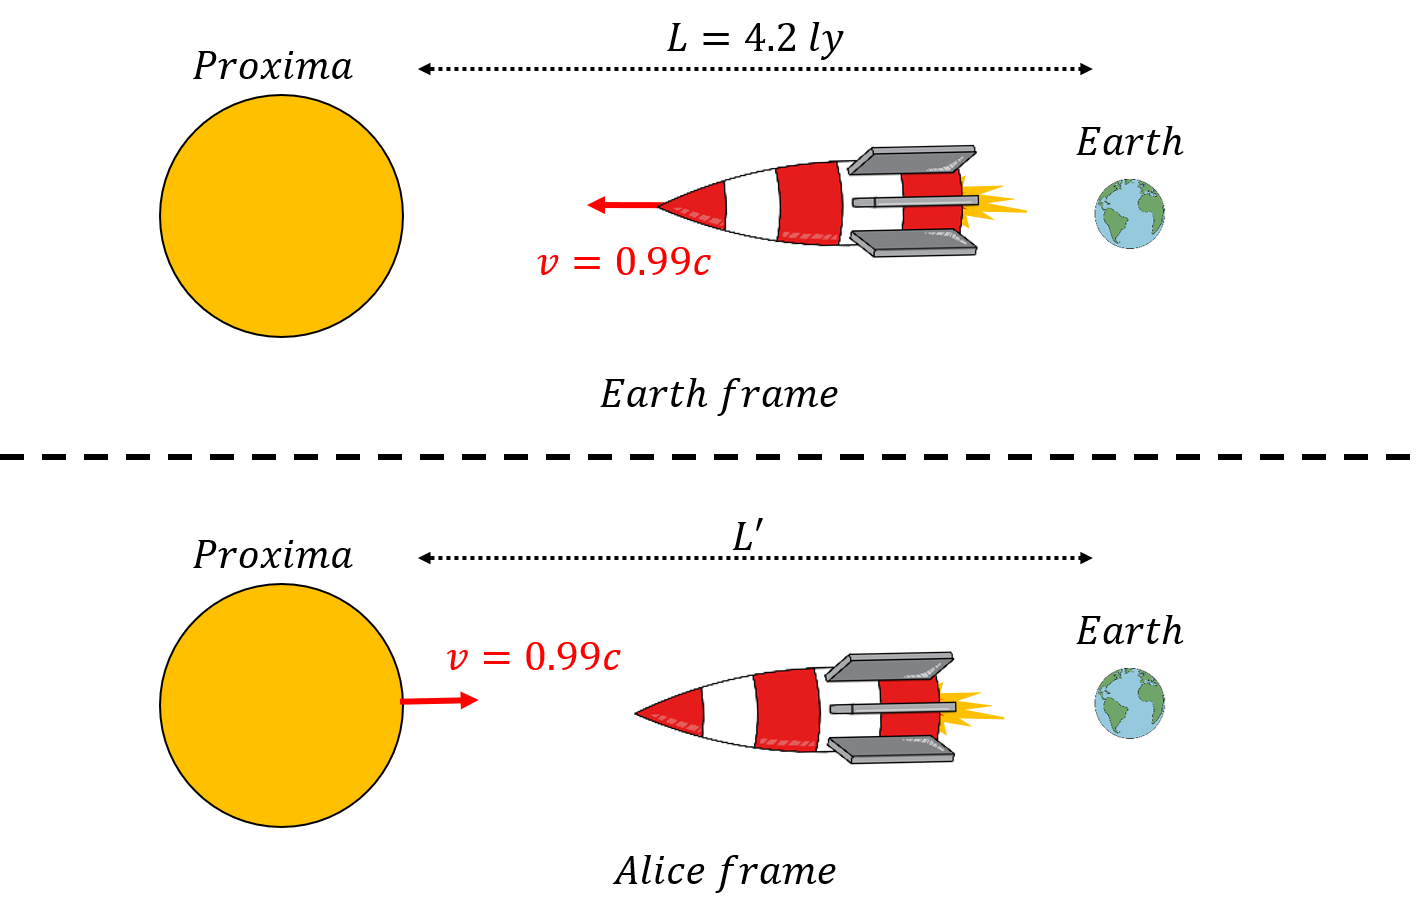
\includegraphics[width=0.8\linewidth]{files/alphatrip-3ea02d44948e5bb04a3cc62ada80ac9a.png}
\caption[]{Alice travels in a spaceship from the Earth to the star Proxima Centauri. In the Earth frame of reference, the star is $4.2 {\rm ly}$ away.}
\label{fig:specialrelativity:alphatrip}
\end{figure}

\begin{framed}
\textbf{Solution}\\
In Earth's frame of reference, the spaceship travels a distance of $4.2 {\rm ly}$ at a speed of $0.99c$, which will take a time, $\Delta t'$, given by:
\begin{equation}
\Delta t' = \frac{(4.2 {\rm ly})}{(0.99c)}=4.2 {\rm y}
\end{equation}
which is not surprising, since Alice is travelling at almost the speed of light. This is the time that goes by on planet Earth. Since Alice's spaceship is moving, less time will go by on the spaceship, as the $4.2 {\rm y}$ is the dilated time measured at Earth, not the proper time measured by Alice. First, we determine the gamma factor:
\begin{equation}
\gamma = \frac{1}{\sqrt{1-\frac{v^2}{c^2}}} =\frac{1}{\sqrt{1-0.99^2}}=7.1
\end{equation}
The proper time measured by Alice is:
\begin{equation}
\Delta t = \frac{\Delta t'}{\gamma}=\frac{(4.2 {\rm y})}{(7.1)}=0.6 {\rm y}
\end{equation}
That is, Alice only ages by $0.6 {\rm y}$ (about 7 months), while everyone on Earth ages by $4.2 {\rm y}$!In Alice's frame of reference, she is not moving, and Proxima Centauri moves towards her at a speed of $0.99c$. Since her trip only lasts about 7 months ($0.6 {\rm y}$), Proxima Centauri moves towards her by a distance, $L'$:
\begin{equation}
L'=v\Delta t=(0.99c)(0.6 {\rm y})=0.6 {\rm ly}
\end{equation}
as illustrated in Figure~\ref{fig:specialrelativity:alphatrip}. Thus, Alice concludes that the distance between Earth and Proxima Centauri is only $0.6 {\rm ly}$ instead of $4.2 {\rm ly}$. The distance that she observes is contracted compared to the ``proper distance'' between Earth and Proxima (the distance measured when we are at rest relative to Earth and Proxima).

\textbf{Discussion:} In this example we saw, again, how the time that one measures depends on the frame of reference. In particular, if one can build spaceships that goes close to the speed of light, one can cover large distances in the Universe without ageing much. We also saw that length contraction is a necessary corollary to time-dilation. Objects appear contracted when they move, relative to their length when they are measured at rest (their ``rest length'' or their ``proper length'').
\end{framed}
\end{framed}

One interesting issue uncovered by Example~23.2 is the so-called ``twin-paradox''. Imagine that Alice has a twin brother, Brice, that remains on Earth. Alice travels to Proxima Centauri and back (return trip), and will have aged by about 14 months, whereas Brice, will have aged by about 8.4 years (using the numbers in Example~23.2). However, Einstein's first postulate implies that there are no special frames of reference that are at rest. We should be able to think about this situation from the perspective where Alice is at rest, and it is the Earth (with Brice on it), that moves away from her and then back. In this case, Alice is at rest, and she will conclude that it takes about 8.4 years for Brice to move away and come back, and that Brice would have aged by about 7 months. When Alice and Brice meet up again, clearly Alice cannot be both younger and older than Brice, so which one is it? (You will have to look this up, see associated question in the ``Thinking about the material'' section).

\subsubsection{Length contraction}

As we saw in the examples from the previous section, time dilation implies ``length contraction''. When an object is measured in a frame of reference that is at rest relative to the object, the length of the object, $L$, is called the ``rest length'' or the ``proper length'' of the object. If that object is moving relative to an observer, the observer will measure the object to be shorter, and have a ``contracted length'', $L'$, given by:
\begin{equation}
\boxed{L'=L\sqrt{1-\frac{v^2}{c^2}} =\frac{L}{\gamma}}
\end{equation}
In Example~23.2, Alice measured a contracted distance between Earth and Proxima Centauri, as she was in a frame of reference that is moving relative to the Earth-Proxima Centauri reference frame. One point that is important to note is that length contraction only occurs along the direction parallel to the direction of motion.

\begin{framed}
\textbf{Example 23.3}\\
A square painting hanging in a museum has a side with a length of $1 {\rm m}$. If you view the stationary painting from a train moving in the horizontal direction at a speed of $0.85c$, what is the surface area of the painting that you measure?

\begin{framed}
\textbf{Solution}\\
Since your train is moving horizontally, only the horizontal dimension of the painting will be contracted. The gamma factor is given by:
\begin{equation}
\gamma = \frac{1}{\sqrt{1-\frac{v^2}{c^2}}} =\frac{1}{\sqrt{1-0.85^2}}=1.9
\end{equation}
Thus, the horizontal side of the painting will have a contracted length:
\begin{equation}
L'=\frac{L}{\gamma}=\frac{(1 {\rm m})}{(1.9)}=0.53 {\rm m}
\end{equation}
The area of the painting, as measured in the moving frame of reference, is given by:
\begin{equation}
A= (1 {\rm m})(0.53 {\rm m})=0.53 {\rm m^2}
\end{equation}
\end{framed}
\end{framed}

\begin{framed}
\textbf{Checkpoint}\\
At what speed must an object travel in order for it to appear 1\% shorter?

\begin{enumerate}
\item $0.01c$
\item $0.04c$
\item $0.99c$
\item $0.65c$
\end{enumerate}

\begin{framed}
\textbf{Answer}\\
\begin{enumerate}[resume]
\item
\end{enumerate}
\end{framed}
\end{framed}

\begin{framed}
\textbf{Olivia's Thoughts}\\
In these types of problems, it is important to keep track of which reference frame gives us the proper length and which gives us the proper time. I recommend taking a minute at the beginning of each problem to think about this, and jot it down at the start of your solution. Take Figure~\ref{fig:specialrelativity:alphatrip}, in which our friend Alice travels from Earth to Proxima Centuri on a spaceship. We are dealing with Earth's frame of reference, which I will call $E$, and the Alice's frame of reference, which I will call $A$. We are interested in the time elapsed on the spaceship and the distance to Proxima Centuri. The Earth is \textit{moving} relative to the spaceship's clock and is \textit{stationary} relative to Proxima Centuri. Thus, frame $E$ gives us the \textit{dilated time}, $\Delta t'$, and the \textit{proper length}, $L$. Alice is \textit{stationary} relative to the spaceship's clock and is \textit{moving} relative to Proxima Centuri. Thus, frame $A$ gives us the \textit{proper time}, $\Delta t$, and the \textit{contracted length}, $L'$.\newline
At the top of my solution, I would write:
\begin{equation}
\textrm{Frame}\, E: L, \Delta t'\\
\textrm{Frame}\, A: L', \Delta t
\end{equation}
To check that we got this right, the speed of the spaceship should not change depending on the reference frame. In the Earth's frame of reference, the velocity is given by $v=L/\Delta t'$. In Alice's frame, it is given by $v=L'/\Delta t$, or, using the gamma factor:  $v=(L/\gamma)/(\Delta t'/\gamma)=L/\Delta t'$, as expected.
\end{framed}

Length contraction also allows us to discuss a famous paradox (the ``barn'', or ``ladder'' or ``barn-pole'' paradox). Consider a train that has a rest length of $500 {\rm m}$, travelling at a speed such that $\gamma = 2.5$. As the train goes by, from Earth, it appears to have a (contracted) length:
\begin{equation}
L'_{train}=\frac{(500 {\rm m})}{2.5}=200 {\rm m}
\end{equation}

Suppose that there is a tunnel on Earth that is exactly $200 {\rm m}$ long, so that the train, when contracted, will fit in the tunnel. When the train passes, an operator briefly closes (and re-opens) the doors at the ends of the tunnel, briefly ``capturing'' the train, and since the train is contracted, it never hits any of the doors, and all is fine.

From the train's frame of reference, the train has a proper length of $500 {\rm m}$, and the tunnel is contracted to a length of:
\begin{equation}
L'_{tunnel}=\frac{(200 {\rm m})}{(2.5)}=80 {\rm m}
\end{equation}
Thus, from the train's perspective, if the doors of the tunnel are closed, there is no way that the $500 {\rm m}$ long train can ever fit in the $80 {\rm m}$ long tunnel, as illustrated in Figure~\ref{fig:specialrelativity:barn}. So what happens when the operator on Earth closes the doors of the tunnel to briefly ``capture'' the train?

\begin{figure}[!htbp]
\centering
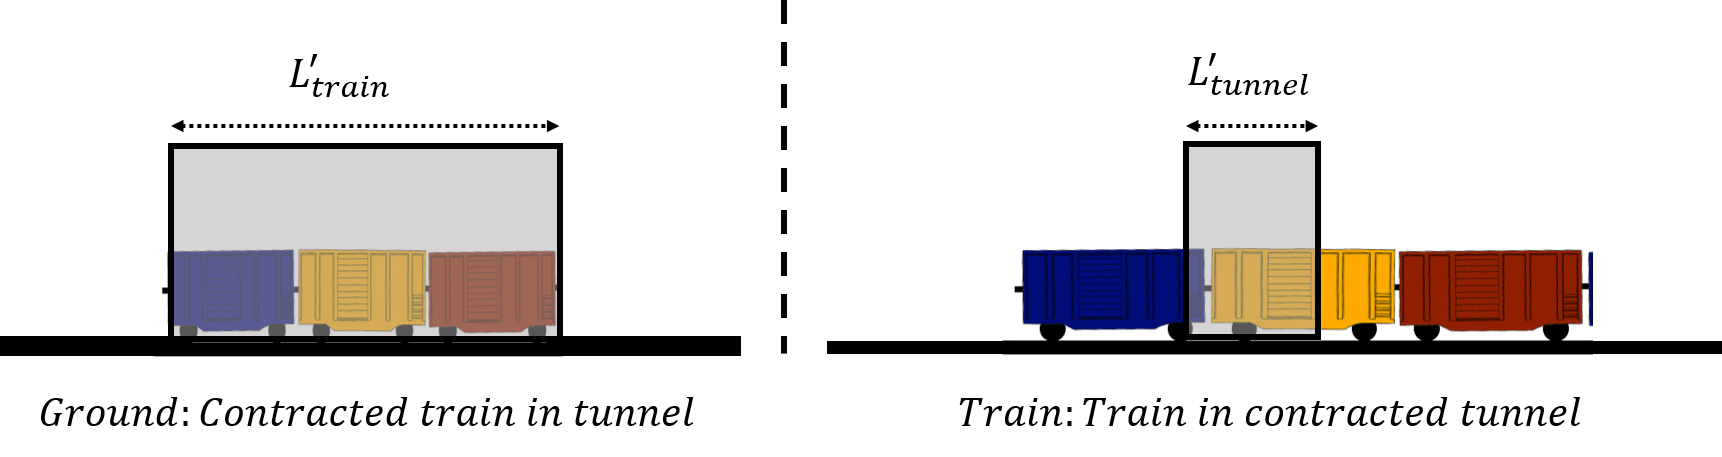
\includegraphics[width=0.8\linewidth]{files/barn-445f4a4d750354c503a5ac61fc0d77e9.png}
\caption[]{In the ground's reference frame, the contracted train appears to fit inside the tunnel. From the train, the (proper length) train will not fit in the contracted tunnel.}
\label{fig:specialrelativity:barn}
\end{figure}

Clearly, people on the Earth and people on the train have to agree on whether the train was destroyed by the tunnel doors. The operator on Earth can clearly close both doors of the tunnel when the train is inside and not destroy the train. Hence, people on the train must agree that the train never collided with the doors, and that the doors were closed. The answer to this paradox lies in the fact that simultaneity is relative. The tunnel operator believes that she has closed the two doors of the tunnel at exactly the same time, precisely when the contracted train is lined up with the tunnel. However, to people on the train, in a different frame of reference, the doors did not close at the same time, since events that are simultaneous in one frame of reference are not necessarily simultaneous in a different frame of reference. To people on the train, there was never a time when the train was in the tunnel and both doors were closed at the same time!

\begin{framed}
\textbf{Checkpoint}\\
Referring to the above paradox, to people on the train, which tunnel door closes first?

\begin{enumerate}
\item The door at the entrance of the tunnel closes first.
\item The door at the exit of the tunnel closes first.
\end{enumerate}

\begin{framed}
\textbf{Answer}\\
\begin{enumerate}[resume]
\item
\end{enumerate}
\end{framed}
\end{framed}

\subsubsection{Electric and magnetic fields and Special Relativity}

In this section, we present one more example to show how Special Relativity is connected to electromagnetism. Consider a wire that carries an electric current towards the left, and a positive charge, $+Q$, located next to the wire, as illustrated in Figure~\ref{fig:specialrelativity:current}.

\begin{figure}[!htbp]
\centering
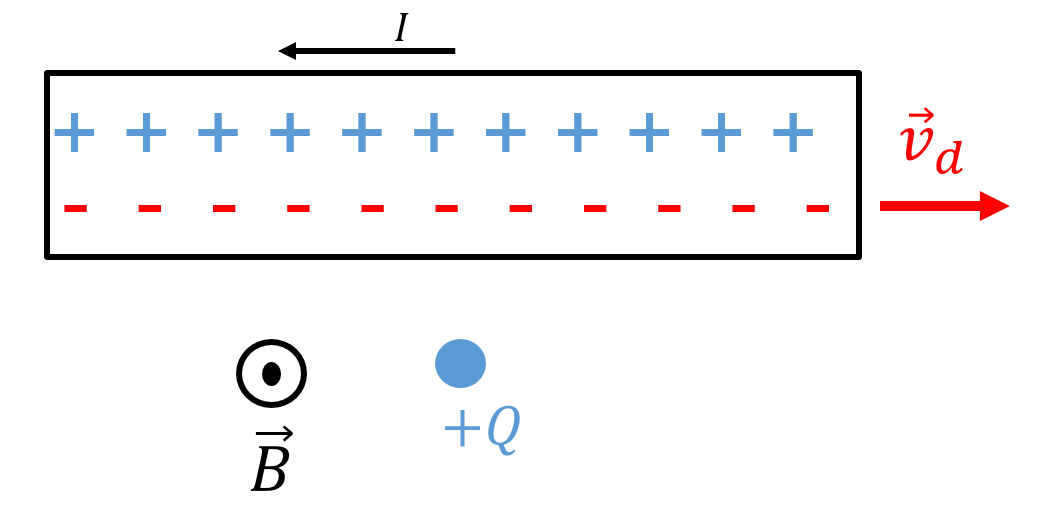
\includegraphics[width=0.5\linewidth]{files/current-08fd956639cd7f7deeb7878bc82f3d20.png}
\caption[]{A stationary positive charge, $+Q$, near a wire carrying current towards the left. This leads to a magnetic field out of the page at the location of $Q+$.}
\label{fig:specialrelativity:current}
\end{figure}

Inside the wire, negative electrons are moving towards the right with a drift velocity, $\vec v_d$, while positive ions remain stationary. Since the charge $+Q$ has a velocity of zero, it experiences no magnetic force. Furthermore, the wire appears to be neutral, with no net electric charge.

If the charge, $+Q$, has a velocity, $\vec v_d$, towards the right, it will experience a downwards magnetic force, as illustrated in Figure~\ref{fig:specialrelativity:current_force}.

\begin{figure}[!htbp]
\centering
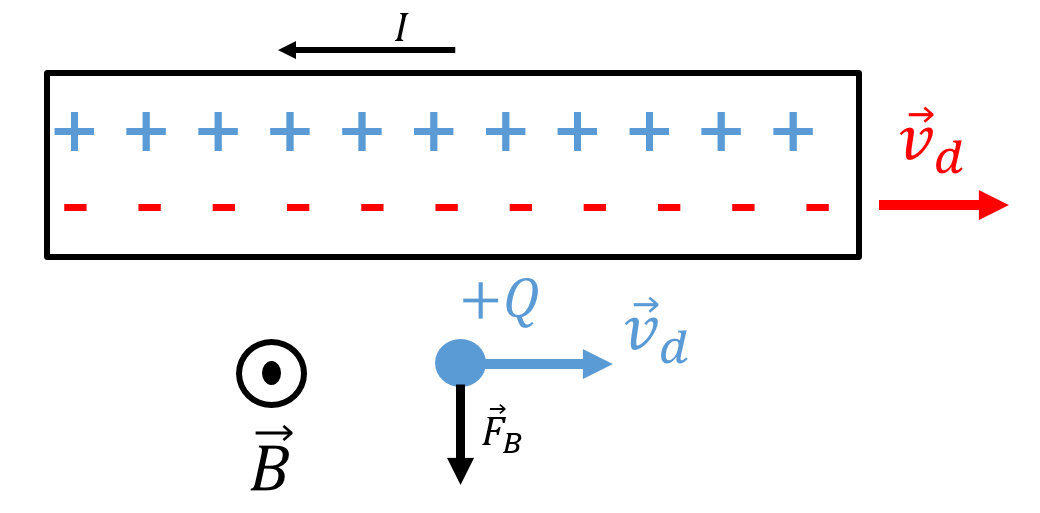
\includegraphics[width=0.5\linewidth]{files/current_force-891d7a63e028add2e0522c709e873359.png}
\caption[]{A positive charge, $+Q$, moving towards the right, near a wire carrying current towards the left, will experience a downwards magnetic force, $\vec F_B=Q \vec v_d\times \vec B$.}
\label{fig:specialrelativity:current_force}
\end{figure}

Now, consider this from the perspective of the charge, $+Q$, as illustrated in Figure~\ref{fig:specialrelativity:current_ions}. The charge $Q$ is moving towards the right at the same speed as the electrons in the wire. In the reference frame of the charge, $+Q$, the charge has a velocity of zero, and thus will experience no magnetic force. The wire still appears to have a (different) current, $I'$, as the positive ions move to the left, creating a magnetic field, $\vec B'$, out of the page.

In the ``lab'' frame of reference, where the electrons and the charge $+Q$ move towards the right at the same speed, $v_d$, the electrons appear closer together (length contracted) than they are in the frame of reference of the electrons (or of the charge $+Q$, since it is moving with the electrons). In the frame of reference of the charge $+Q$, the electrons thus appear to be spaced further apart (less dense). On the other hand, in the frame of reference of $+Q$, the positive ions, which are moving towards the left, appear closer together, as the distance between them is now contracted, as illustrated in Figure~\ref{fig:specialrelativity:current_ions}.

\begin{figure}[!htbp]
\centering
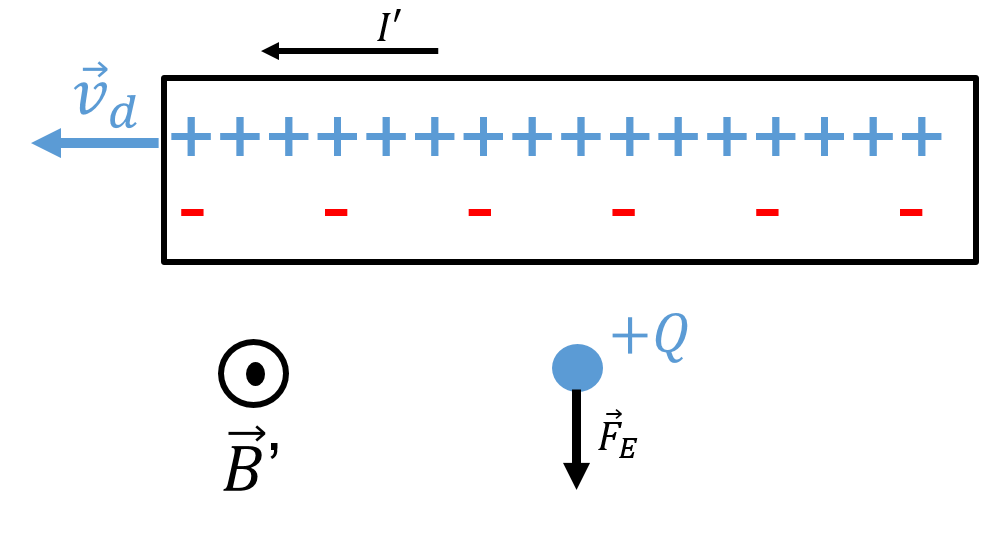
\includegraphics[width=0.5\linewidth]{files/current_ions-de3896591af7b6dd91be2e91dddf5da7.png}
\caption[]{In the frame of reference of the charge $+Q$, the charge has a velocity of zero and cannot experience a magnetic force. The ions appear to move to the left, and thus appear denser, since the distance between ions is contracted. The distance between electrons, on the other hand, is larger in this frame of reference. It thus appears that the wire is positively charged, and would exert a downwards electric force on the charge, $+Q$.}
\label{fig:specialrelativity:current_ions}
\end{figure}

In the frame of reference of the charge $+Q$, the wire no longer appears neutral, but appears to have a net positive charge. This results in an electric field away from the wire that will exert a downwards force on $+Q$. In both frames of reference, we conclude that the charge will experience a downwards force. Whether that force is magnetic or electric depends on the frame of reference! Here, we came to the conclusion by using the notion of length contraction, but remember that length contraction itself is a consequence of Maxwell's equations holding in different frames of reference, as we illustrated at the beginning of this chapter.

In most real-world applications, we do not see the effects of Special Relativity, as the speeds involved must be very high for the gamma factor to be appreciably greater than one. However, we see these effects in electromagnetism even though the drift speed of electrons in a wire is usually (much) less than ${\rm mm/s}$. This is because, when dealing with the electric and magnetic forces (fields), even a minuscule length contraction of the electrons/ions at those speeds leads to relativistic effects. This can be thought of in terms of how strong the electric force really is; even a minute change in charge density (due to length contraction) has a sizeable relativistic effect.

\subsubsection{Lorentz transformations and space-time}

% %%Lorentz transformations, space time diagrams

\paragraph{Four-dimensional space-time}

So far, we have seen that our notions of time intervals (the time between two events) and space intervals (the distance between two locations) depend on our frame of reference. We also saw how space and time are connected, for example by the fact that time-dilation must go hand-in-hand with length contraction. Additionally, we concluded that there is no absolute concept of time, and that time is relative.

In the context of Special Relativity, we introduce the concept of space-time. To describe the location of an object in space-time, we must specify both the location/position coordinates ($x$, $y$, $z$) \textbf{and} the time ``coordinate'', $t$. We usually specify the time coordinate by multiplying it by speed of light, $ct$, so that it has dimensions of length rather than time. Thus, position in space-time is given by 4 coordinates: $(x,y,z,ct)$.

\paragraph{Space-time diagrams}

It is practically impossible to visualize situations in three dimensions, so four dimensions is hopeless! However, we can gain a lot of insight into Special Relativity models by using ``space-time diagrams''. In a space-time diagram, we use only one of the space coordinates (typically $x$) along with the time coordinate, $ct$, to define the two axes of a space-time diagram. Space-time diagrams are analogous to ``position as a function of time'' graphs that one would draw in kinematics, although they are fundamentally different in that, for a space-time diagram, the coordinates should be thought of as independent (one is not plotting a dependent variable as a function of an independent variable).

Figure~\ref{fig:specialrelativity:spacetime} shows a space-time diagram for an object that was located at position $x=x_1$ at time $t=t_1$ (location $A$), and at position $x=x_2$ at time $t=t_2$ (location $B$). The path of an object through space-time, indicated by the line that connects $A$ and $B$, is called the ``world line'' of the object.

\begin{figure}[!htbp]
\centering
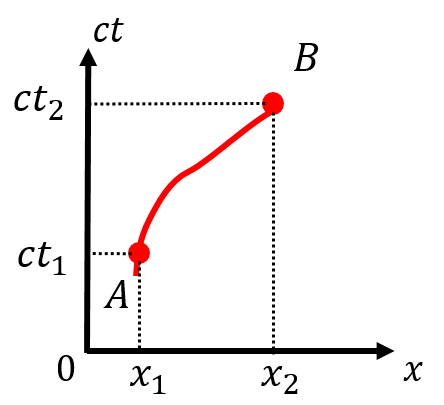
\includegraphics[width=0.5\linewidth]{files/spacetime-42568f401ab38be97970e178fd2c7aed.png}
\caption[]{World line of an object that moved from locations $A$ in space-time to location $B$ in space-time.}
\label{fig:specialrelativity:spacetime}
\end{figure}

\begin{framed}
\textbf{Checkpoint}\\
What does the world-line of a stationary particle look like?

\begin{enumerate}
\item A vertical line.
\item A horizontal line.
\item A point.
\end{enumerate}

\begin{framed}
\textbf{Answer}\\
\begin{enumerate}
\item
\end{enumerate}
\end{framed}
\end{framed}

A pulse of light travelling in the $x$ direction will always have a world-line that makes a $45 {\rm \degree}$ angle with the horizontal (space) axis (since $x=ct$). The world line of any object that travels with a speed below the speed of light must always make an angle with the horizontal axis that is greater than $45 {\rm \degree}$.

A position in space-time is usually called an ``\textbf{event}''. We can draw a set of lines, at $45 {\rm \degree}$ degrees from the horizontal axis, that intersect at an event in space-time. Those lines define two ``light cones'' corresponding to: (1) locations in space-time in the past that could have had a causal effect on the event (the ``past light cone''), and (2), locations in space-time in the future for which the event can have a causal effect (the ``future light cone'').

Figure~\ref{fig:specialrelativity:cones} shows the light cones associated with an event, $A$, in space-time. The past light cone is the only region of space-time in which a different event could have had an impact on the event $A$. For example, the event $A$ might be that ``the object is at position $x=x_1$ at time $t=t_1$'', so that the past light cone corresponds to the only locations in space-time that the object could have been in the past. Similarly, the future light-cone defines the locations in space-time upon which the event $A$ could have an effect. For example, this could define the possible locations of the object in the future. The regions outside the light cones can never have an effect on the event $A$; they are not causally connected. A signal or object would need to travel faster than the speed of light in order to have an effect on something outside of its light cone. There are locations in space-time, in the future of our Universe, that we cannot influence, no matter what we do.

\begin{figure}[!htbp]
\centering
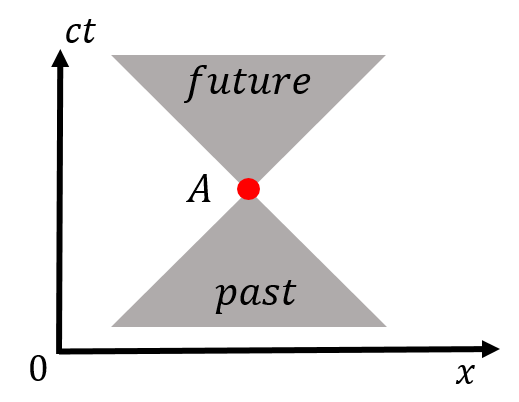
\includegraphics[width=0.5\linewidth]{files/cones-c0bdfac7e214c550281ebd9da604b0f5.png}
\caption[]{The past and future light cones associated with the space-time event, $A$.}
\label{fig:specialrelativity:cones}
\end{figure}

When two events in space-time are within each other's light cones, we say that the space-time interval between them (the line that you draw from one event to the other) is ``time-like''. Time-like events are such that all observers, in any frame of reference, will agree that one event happened before the other. Thus, events that are causally related must have a time-like interval between them (they are connected by a line that makes an angle greater than $45 {\rm \degree}$ with the horizontal axis).

Two events that are outside of each other's light cones are said to be ``space-like''. Events that are connected by space-like intervals cannot be causally related (one cannot cause the other). Observers in different frames of reference will disagree on the time ordering of space-like events. For example, when Alice observed the two clocks on the platform to emit pulses of light at the same time, Brice disagreed; those two events are connected by a space-like interval.

Finally, the space-time interval between events that are on each other's light-cone (connected by a line that makes a $45 {\rm \degree}$ angle with the x-axis), is said to be ``light-like'' or ``null''.

\paragraph{Lorentz transformations}

In this section, we consider how to transform the space-time coordinates, $(x,y,z,ct)$, as measured in a frame of reference, $S$, to coordinate $(x',y',z',c't)$, as measured in a frame of reference, $S'$, that is moving with a constant speed, $v$, relative to the frame, $S$. For simplicity, we assume that frame $S'$ is moving with speed $v$ in the positive $x$ direction, as measured in frame, $S$, and that the origin of the two coordinate systems coincided at time $t=0$. Figure~\ref{fig:specialrelativity:translation} shows an illustration of how the two frames of reference are related (note that these are actual coordinate systems, not space-time diagrams).

\begin{figure}[!htbp]
\centering
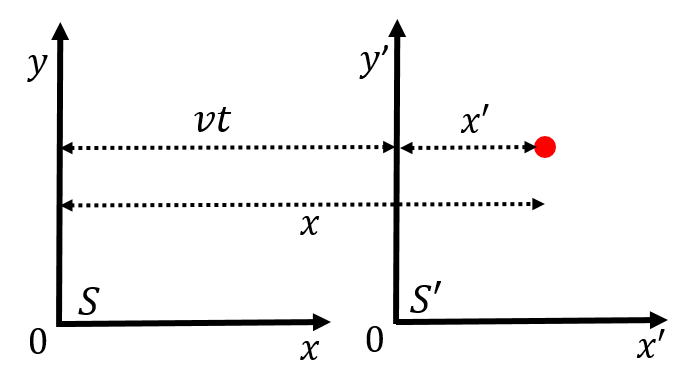
\includegraphics[width=0.5\linewidth]{files/translation-645d294e4cbfefbcdd841cbac530336d.png}
\caption[]{The reference frame $S'$ is moving relative to reference frame, $S$, with speed $v$ in the $x$ direction. At time $t=0$, the origins of the two coordinate systems coincided.}
\label{fig:specialrelativity:translation}
\end{figure}

If we ignore any of Special Relativity, then the coordinates in $S'$ are easily related to those in the $S$ frame of reference using the ``Galilean transformations'':
\begin{equation}
x' &= x - vt\\
y' &= y\\
z' &= z\\
t' &= t
\end{equation}
and this corresponds to transformations that we have implicitly used before considering Special Relativity. These equations also allow us to relate the speeds measured in different frames of reference. Suppose that an object has a velocity, $\vec u=(u_x,u_y,u_z)$, as measured in the frame of reference, $S$. We can obtain the components of the velocity vector, $\vec u'$, as measured in the frame of reference, $S'$, by taking the time derivatives of the above equations:
\begin{equation}
u'_x &= \frac{dx'}{dt'}=\frac{dx'}{dt}=\frac{d}{dt}(x-vt)=\frac{dx}{dt}-v=u_x - v\\
u'_y &=\frac{dy'}{dt'}=u_y\\
u'_z &=\frac{dz'}{dt'}=u_z
\end{equation}
which is trivial, since $t=t'$. The transformations above are equivalent (identical) to the rules for transforming velocity that we derived in \href{\#sec:describingmotionin1D:relativemotion}{Section  \%s} for kinematics. In Galilean relativity, time is an absolute quantity that does not depend on the frame of reference. In Special Relativity, the time coordinate depends on the frame of reference, so we cannot simply convert a time derivative in $t'$ to a derivative in $t$. Instead, we must use the Lorentz transformations.

We can use the formulas for length contraction and time dilation to derive the Lorentz transformations. Referring to Figure~\ref{fig:specialrelativity:translation}, $x$ refers to the distance between a point in space-time and the origin of the $x$ axis in frame $S$, as measured in frame $S$. Similarly, $x'$, is the distance to the point in space-time as measured in frame $S'$, from the origin of $S'$. In frame  $S$, the distance $x'$ will be contracted to the length $x'/\gamma$, so that the Galilean transformation for the $x$ coordinate is modified as follows:
\begin{equation}
x' &= x - vt\quad\text{(Galilean)}\\
\frac{x'}{\gamma} &= x - vt\\
\therefore x'&=\gamma (x-vt)\quad\text{(Lorentz)}
\end{equation}
The $y$ and $z$ coordinates are the same between frames of references, since all of the length contraction will take place in the direction of the relative motion between frames of reference, which we chose to be in the $x$ direction.

We can obtain the equation for the time coordinate by considering that, in the $S'$ frame of reference, it is the $x$ coordinate that is contracted to $x/\gamma$. In the $S'$ frame of reference, the distance between the origins of the two systems is $vt'$ (note the prime on $t$). We can thus write the contracted distance $x$, in the $S'$ frame of reference:
\begin{equation}
\frac{x}{\gamma}&=vt'+x'\\
t'&= \frac{1}{v}\left(\frac{x}{\gamma}-x'\right)
\end{equation}
We can eliminate $x'$ from the last equation using the Lorentz transformation for $x'$ that we just found:
\begin{equation}
t'&= \frac{1}{v}\left(\frac{x}{\gamma}-x'\right)\\
t'&= \frac{1}{v}\left(\frac{x}{\gamma}-\gamma x+\gamma vt\right)\\
\frac{t'}{\gamma}&=\frac{1}{v}\left(\frac{x}{\gamma^2}-x+vt\right)\\
&=\frac{1}{v}\left(x\left(1-\frac{v^2}{c^2}\right)-x+vt\right)\\
&=\frac{1}{v}\left(-\frac{v^2}{c^2}x+vt\right)\\
&=t-\frac{vx}{c^2}\\
\therefore t'&=\gamma\left(t-\frac{vx}{c^2} \right)
\end{equation}
where we wrote out the $\gamma$ factor out explicitly in the fourth line. We can summarize the Lorentz transformations as follows:
\begin{equation}
x' &=\gamma (x-vt)\\
y' &= y\\
z' &= z\\
t' &=\gamma\left(t-\frac{vx}{c^2} \right)
\end{equation}
and the inverse relations are easily found:
\begin{equation}
x &=\gamma (x'+vt')\\
y &= y'\\
z &= z'\\
t &=\gamma\left(t'+\frac{vx'}{c^2} \right)
\end{equation}
Note that the Lorentz transformations reduce to the Galilean transformations when the speed, $v$, between frames of reference is small (so that $\gamma \sim 1$).

\begin{framed}
\textbf{Example 23.4}\\
In a frame, $S$, a pulse of light is emitted (at the speed of light) in the positive $x$ direction at $t=0$ from the origin. The pulse is then absorbed at time $t$ at position $x=d$. Use the Lorentz transformation to show that, in a frame, $S'$, moving in the positive $x$ direction with speed $v$, relative to $S$, the pulse also travelled at the speed of light.

\begin{framed}
\textbf{Solution}\\
In order to use the Lorentz transformations, we need to define ``events'', with coordinates in space-time, that we can then convert from one frame of reference to another. Let $A$ be the event that corresponds to the emission of the pulse of light, and $B$ the event that corresponds to the absorption of the pulse. In frame, $S$, the coordinates of these events are:
\begin{equation}
x_A&=0\\
t_A&=0\\
x_B&=d\\
t_B&=\frac{d}{c}
\end{equation}
where in the last line, we used the fact that, in frame, $S$, the pulse travels at the speed of light. Applying the Lorentz transformations, we can find the coordinates of the same events in frame $S'$:
\begin{equation}
x'_A&=\gamma (x_A-vt_A)=0\\
t'_A&=\gamma\left(t_A-\frac{vx_A}{c^2} \right)=0\\
x'_B&=\gamma (x_B-vt_B)=\gamma \left(d-v\frac{d}{c}\right)\\
t'_B&=\gamma\left(t_B-\frac{vx_B}{c^2} \right)=\gamma\left(\frac{d}{c}-\frac{vd}{c^2} \right)
\end{equation}
The speed, $v'_p$, of the pulse of light in frame $S'$ is given by:
\begin{equation}
v'_p&=\frac{(x'_B-x'_A)}{(t'_B-t'_A)}=\frac{\gamma \left(d-v\frac{d}{c}\right)}{\gamma\left(\frac{d}{c}-\frac{vd}{c^2} \right)}\\
&=\frac{\left(d-v\frac{d}{c}\right)}{\left(\frac{d}{c}-\frac{vd}{c^2} \right)}=c\frac{\left(\frac{d}{c}-v\frac{d}{c^2}\right)}{\left(\frac{d}{c}-\frac{vd}{c^2} \right)}=c
\end{equation}
which is the speed of light, as expected.

\textbf{Discussion:} In this example, we showed how to use the Lorentz transformations by clearly defining ``events'' and their coordinates in space-time. We saw that the Lorentz transformations are consistent with Einstein's second postulate and that the speed of light is the same all frames of reference. This of course makes sense, as we derived the Lorentz transformations from time dilation and length contraction, which are consequences of the postulate.
\end{framed}
\end{framed}

Einstein's second postulate states that the speed of light is independent of the frame of reference. Consider two points in space-time corresponding to the emission ($A$) and the absorption ($B$) of a pulse of light. In the reference frame, $S$, the distance squared in space between these two events must be equal to the distance (squared) that light travelled between the time of emission and absorption:
\begin{equation}
(x_B-x_A)^2+(y_B-y_A)^2+(z_B-z_A)^2&= c^2(t_B-t_A)^2\\
\therefore \Delta x^2 + \Delta y^2 +\Delta z^2&=c^2\Delta t^2
\end{equation}
where $(x_A,y_A,z_A,ct_A)$ and $(x_B,y_B,z_B,ct_B)$ are the space-time coordinates of events $A$ and $B$. The above equation must hold in all frame of references (e.g. adding a prime to each coordinate), since it is a statement that the speed of light is $c$.

We can define $s$ as the ``space-time interval'' between events $A$ and $B$:
\begin{equation}
s^2 = \Delta x^2 + \Delta y^2 +\Delta z^2&-c^2\Delta t^2
\end{equation}
which turns out to be ``Lorentz invariant'' (meaning that this value is the same in all reference frames). The space-time interval can be thought of as a ``distance'' in space-time that is the same in all reference frames. If the events $A$ and $B$ corresponds to the emission and absorption of light, then $s=0$, and we say that the interval between $A$ and $B$ is light-like or null. If $s<0$, the events are on a time-like interval, and if $s>0$, the events are separated by a space-like interval. Since $s$ does not depend on the frame of reference, all observers will agree on whether events are separated by time or space-like intervals.

We can visualize the effect of Lorentz transformations on space-time diagrams, as in Figure~\ref{fig:specialrelativity:lorentz}, which shows the space-time diagrams for a reference frame, $S$, and a second reference frame, $S'$, moving with speed $v$ in the $x$ direction relative to $S$.

\begin{figure}[!htbp]
\centering
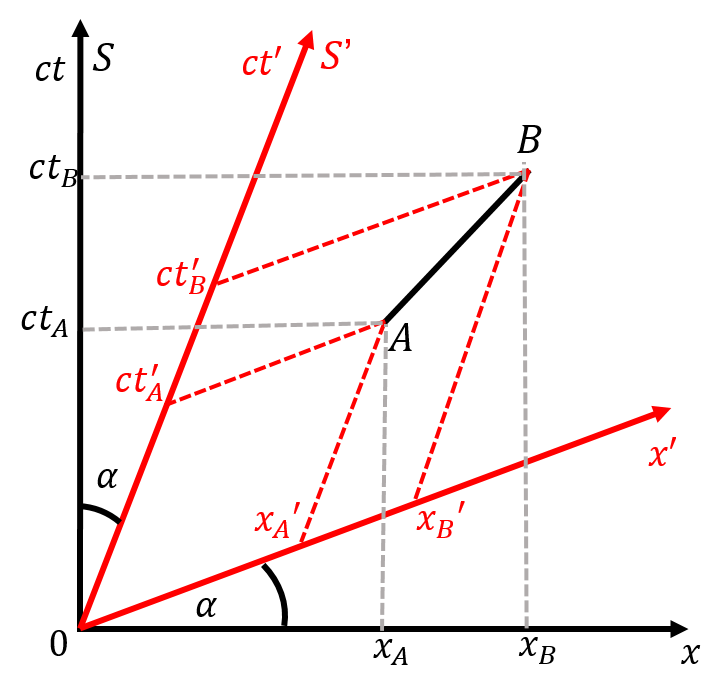
\includegraphics[width=0.6\linewidth]{files/lorentz-f7121c5a4528f9422e6c506f6f1a6d4b.png}
\caption[]{The reference frame $S'$ is moving relative to reference frame, $S$, with speed $v$ in the $x$ direction. We can illustrate this on a space-time diagram by tilting the axes of the $S'$ coordinate system by an angle $\tan\alpha=v/c$, as shown.}
\label{fig:specialrelativity:lorentz}
\end{figure}

The effect of the Lorentz transformation on a space-time diagram is to tilt both the space and time axes ``inwards''\footnote{Outwards if the speed of $S'$ is in the negative $x$ direction relative to $S$.}, by an angle, $\alpha$, given by:
\begin{equation}
\tan\alpha = \frac{v}{c}
\end{equation}
Figure~\ref{fig:specialrelativity:lorentz} shows a light-like interval between two points, $A$ and $B$, and how to determine the space-time coordinates in the two reference frames. You can think of space-time as the sheet of paper on which events happen. You can then draw different coordinate systems on that piece of paper to describe the position (in space and time) of different events.

\begin{framed}
\textbf{Example 23.5}\\
Use a space-time diagram to show how two events at different locations that are simultaneous in one frame of reference are not simultaneous in a reference frame that is moving relative to the one where the events are simultaneous. This is an illustration of the relativity of simultaneity that we uncovered at the beginning of the chapter when examining Alice on a train platform and the two pulses of light.

\begin{framed}
\textbf{Solution}\\
Let $S$ be the frame of reference where two events, $A$ and $B$, are simultaneous. These events are connected by a space-like interval, since they are separated in space, but not in time. There is no way for one event to have caused the other. In frame $S$, these events are on a horizontal line in a space-time diagram.

Let us define a second reference frame, $S'$, that is moving with speed $v$, relative to $S$. We have illustrated space-time diagrams for the the two reference frames and the events $A$ and $B$ in Figure~\ref{fig:specialrelativity:lorentz_simul}.

\begin{figure}[!htbp]
\centering
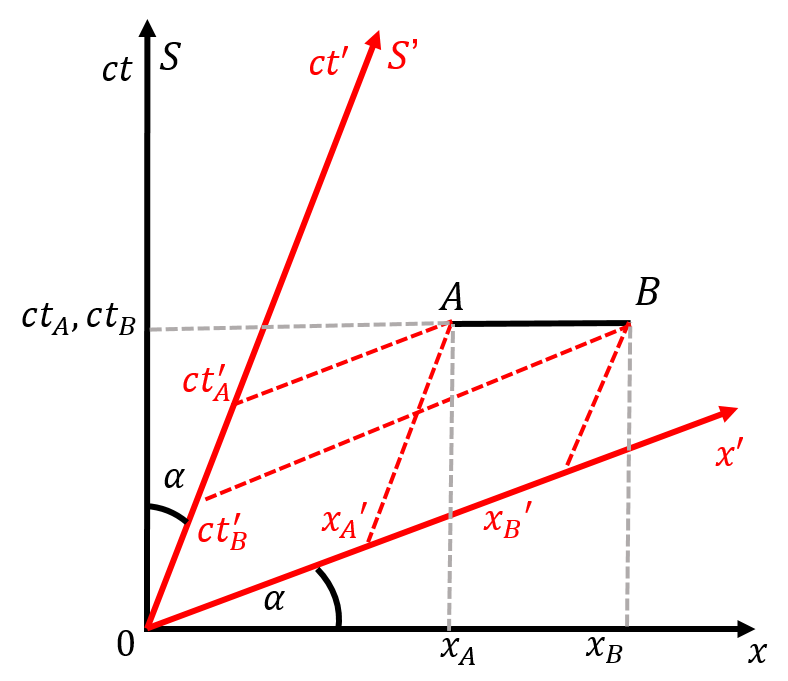
\includegraphics[width=0.6\linewidth]{files/lorentz_simul-dcb660c94da845ad6c4d1a23e49fe632.png}
\caption[]{In the frame of reference $S$, the events $A$ and $B$ occur at the same time. In frame, $S'$, event $B$ occurs before event $A$ (since $t_B < t_A$). The two events are space-like, so observers in different frames of reference cannot agree on which happened first.}
\label{fig:specialrelativity:lorentz_simul}
\end{figure}

From the space-time diagram, it is clear that, in frame $S'$, event $B$ happened first. If frame $S'$ was moving in the opposite (negative $x$) direction, event $A$ would occur first, and the axes of $S'$ would be tilted in the other direction (so that the opening angle between the axes is greater than $90 {\rm \degree}$).

\textbf{Discussion:} This example illustrates how space-time diagrams can be used to qualitatively model events in space-time between two different reference frames. In particular, we showed how two events that are simultaneous in one frame ($S$) are not simultaneous in a different frame. For events connected by space-like intervals, there exist frames of reference where the events are simultaneous, or where either one happened first. If two events are separated by a time-like interval, there is no frame of reference in which one will disagree in the ordering of the events (although observers in different frames of reference will still measure different lengths of time between events due to time-dilation). For time-like events, the moving frame of reference would have to go faster than the speed of light for the time ordering to be different. This would violate causality, and is a good argument as to why nothing can go faster than the speed of light!
\end{framed}
\end{framed}

\begin{framed}
\textbf{Olivia's Thoughts}\\
Now that we know how to visualize Lorentz transformations on space time diagrams, we can better understand space-like and time-like events. In the left panel of Figure~\ref{fig:specialrelativity:spacetimelike}, I have shown an event $A$ and its light cone. Events $A$ and $B$ are space-like, because they are separated more in space than in time (we can see this from the slope: the rise is less than the run). Conversely, events $A$ and $C$ are time-like because they are separated more in time than space. None of these three events occur at the same time or place in this reference frame.

\begin{figure}[!htbp]
\centering
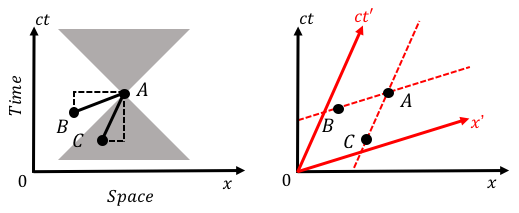
\includegraphics[width=0.8\linewidth]{files/spaceliketimelike-6bcf172ccd155ee5d3ea785d3705d79f.png}
\caption[]{Left: Three events, $A$, $B$, and $C$, that are separated in space and time. We can determine if the intervals between them are space-like or time-like by looking at the slope and comparing the rise and the run. Right: In a new reference frame, events $A$ and $B$ occur at the same time and events $A$ and $C$ occur at the same place.}
\label{fig:specialrelativity:spacetimelike}
\end{figure}

In the right panel of Figure~\ref{fig:specialrelativity:spacetimelike}, I have introduced a new reference frame. You can see that in the new reference frame, events $A$ and $B$ occur at the same time (they are connected by a line that is parallel to the $x'$ axis), and events $A$ and $C$ occur at the same position. In this example, I have shown that if the interval between two events is space-like (e.g. for $A$ and $B$), there is a reference frame in which they occur at the same time. Similarly, if the interval is time-like (e.g. for $A$ and $C$), there is a reference frame in which they occur at the same place.
\end{framed}

\paragraph{Lorentz addition of velocities}

In the previous section, we reviewed the Galilean velocity transformations that allow us to convert a velocity, $\vec u$, as measured in one frame of reference, to a velocity, $\vec u'$, measured in a different frame of reference. We now derive the equivalent relations based on the Lorentz transformation. Again, we assume that frame $S'$ moves in the positive $x$ direction with speed $v$, relative to frame $S$.

The $x$ component of the velocity vector, $\vec u'$, for some object in the $S'$ frame of reference is given by:
\begin{equation}
u'_x = \frac{d}{dt'} x'
\end{equation}
In Galilean relativity, we could simply replace the derivative over $t'$ by a derivative over $t$, since the two are equivalent. This is no longer the case. However, we can use the chain rule and the Lorentz transformations to convert a derivative over $t'$ to a derivative over $t$:
\begin{equation}
\frac{d}{dt'} &= \frac{dt}{dt'}\frac{d}{dt}\\
&= \frac{d}{dt'} \gamma\left(t'+\frac{vx'}{c^2} \right)\frac{d}{dt}\\
&=\gamma \left(1+\frac{v}{c^2}\frac{dx'}{dt'}\right)\frac{d}{dt}\\
&=\gamma \left(1+\frac{vu'_x}{c^2}\right)\frac{d}{dt}
\end{equation}
where we recognized that $\frac{dx'}{dt'}=u'_x$. The $x$ component of the velocity, as measured in the $S'$ frame of reference, is then given by:
\begin{equation}
u'_x &= \frac{d}{dt'} x'\\
&= \gamma \left(1+\frac{vu'_x}{c^2}\right)\frac{d}{dt}x'\\
&=\gamma \left(1+\frac{vu'_x}{c^2}\right)\frac{d}{dt}\gamma (x-vt)\\
&=\gamma^2 \left(1+\frac{vu'_x}{c^2}\right)(u_x -v)\\
\frac{u'_x}{\gamma^2}&=u_x -v +\frac{vu'_xu_x}{c^2}-\frac{v^2u'_x}{c^2}\\
u'_x\left (1-\frac{v^2}{c^2}\right)&=u_x -v +\frac{vu'_xu_x}{c^2}-\frac{v^2u'_x}{c^2}\\
u'_x \left( 1- \frac{vu_x}{c^2}\right) &=u_x -v
\end{equation}
\begin{equation}
\therefore \; \boxed{u'_x=\frac{u_x -v}{1- \frac{vu_x}{c^2}}}
\end{equation}
where we made use of the Lorentz transformation: $x'=\gamma (x -vt)$. We can proceed in a similar way to determine the $y$ and $z$ components. Note that, unlike the Galilean case, all of the velocity components must transform, since the time derivative is involved for each component. Intuitively, we expect all components of velocity to be affected, since one needs to guarantee that the total speed is always below $c$. The velocity transformations for all components are given by the following:
\begin{equation}
u'_x&=\frac{u_x -v}{1- \frac{vu_x}{c^2}}\\
u'_y &=\frac{u_y}{\gamma\left(1- \frac{vu_x}{c^2}\right)}\\
u'_z &=\frac{u_z}{\gamma\left(1- \frac{vu_x}{c^2}\right)}
\end{equation}
and the reverse transformations are given by:
\begin{equation}
u_x &=\frac{u'_x +v}{1+ \frac{vu_x}{c^2}}\\
u_y &=\frac{u'_y}{\gamma\left(1+ \frac{vu_x}{c^2}\right)}\\
u_z &=\frac{u'_z}{\gamma\left(1+ \frac{vu_x}{c^2}\right)}
\end{equation}
\begin{framed}
\textbf{Example 23.6}\\
An archer can shoot a very fast arrow with a speed of $0.5c$. The archer is on a train moving with speed $v=0.7c$ and fires an arrow in the direction of motion. What is the speed of the arrow, as measured in the frame of reference of the ground?

\begin{framed}
\textbf{Solution}\\
Let the train be the frame of reference, $S'$, moving in the positive $x$ direction with speed $v=0.7c$ relative to the frame, $S$, which corresponds to the ground. The speed of the arrow, as seen from the train ($S'$), is given by:
\begin{equation}
u'_x = 0.5c
\end{equation}
The speed of the arrow, as measured from the ground, is thus given by:
\begin{equation}
u_x &=\frac{u'_x +v}{1+ \frac{vu_x}{c^2}}\\
&=\frac{(0.5c) +(0.7c)}{1+ \frac{(0.7c)(0.5c)}{c^2}}\\`
&=\frac{(1.2c)}{1+(0.7)(0.5)}=\frac{1.2}{1.35}c=0.89c
\end{equation}
\textbf{Discussion:} By using the Lorentz transformations for velocity, we see that the arrow does not exceed the speed of light. Had we used Galilean relativity, we would have concluded that the arrow has a speed of $1.2c$ when measured from the ground.
\end{framed}
\end{framed}

\begin{framed}
\textbf{Josh's Thoughts}\\
This chapter is where the bubble of intuitive reality is popped, and students (like you and me) are given the opportunity to challenge our understanding of how the universe operates. As amazing and exciting as this is, it can also be incredibly frustrating. Many students rely on intuition to guide them as they problem solve, but hit a wall in special relativity. To avoid this issue, I suggest drawing spacetime diagrams and using Lorentz transformations. Practicing with these tools will help make the process of understanding the strange consequences of Einstein's postulates less awkward.

In addition to the practical advice I have given, I recommend embracing the strangeness of reality. Throughout history, scientists have ventured into the unknown in attempts to discover and decode the universe. In many cases, the answer to a question has posed more questions than answers, and humanity is given the opportunity to further understand the world we live in. As a student, you are participating in a process of understanding which allows us to continue the adventure that is scientific inquiry. Confusion can be frustrating, but don't let it discourage you, being confused means that you're only a few steps away from understanding!
\end{framed}

\subsubsection{Relativistic momentum and energy}

In this section, we show how to define momentum and energy in a way that is consistent with the postulates of Special Relativity. We expect that, since time and space depend on the frame of reference of the observer, so too will the momentum and the energy of an object. Consider an object of mass $m_0$, moving in frame of reference $S$, with velocity $\vec u$ (we reserve $\vec v$ to represent the speed between two inertial frames of reference) in the $x$ direction. At some time, $t$, the object will be at position $x$ along the $x$ axis. We define the relativistic momentum as:
\begin{equation}
p = m_0\frac{dx}{dt'}
\end{equation}
where $t'$ is the time as measured in the rest frame of the object. By defining momentum in terms of the proper time of the object, all observers will agree on the value of $t'$. In the frame of reference, $S$, (with time $t$) this corresponds to:
\begin{equation}
p = m_0\frac{dx}{dt'}=m_0\frac{dt}{dt'}\frac{dx}{dt}=m_0\frac{dt}{dt'}u
\end{equation}
where $u$ is the speed of the particle in frame, $S$. We can use time dilation to re-express the derivative:
\begin{equation}
\Delta t &= \gamma \Delta t'\\
\frac{\Delta t}{\Delta t'}&=\gamma\\
\therefore \frac{dt}{dt'}&=\gamma
\end{equation}
where in the last line, we simply took the limit of an infinitesimally short time interval. Therefore, the relativistic momentum of the particle in frame $S$ can be defined as
\begin{equation}
\boxed{\vec p = m_0\gamma\vec u =  \frac{m_0\vec u}{\sqrt{1-\frac{u^2}{c^2}}} }
\end{equation}
where $\gamma$ is calculated with the same speed, $u$, since that is the speed of the reference frame of the object relative to $S$. Note that as the speed, $u$, of the particle approaches the speed of light, the factor of $\gamma$ approaches infinity. This means that an object with a mass can never reach the speed of light, as it would have an infinite momentum. In order to define momentum in a way that resembles the classic definition, one can think of the mass of the object as depending on the speed of the object. We define the rest-mass, $m_0$, of the object as the mass that is measured when the object is at rest. We can then model the mass of the object as increasing with its speed:
\begin{equation}
m(u) = \gamma m_0 = \frac{m_0}{\sqrt{1-\frac{u^2}{c^2}}}
\end{equation}
so that the relativistic momentum would be defined as:
\begin{equation}
\vec p = m(u)\vec u
\end{equation}
In this case, we can think of the mass of the object as increasing with its speed. The object would acquire infinite mass if it were to reach the speed of light.

With the relativistic definition of momentum, Newton's Second Law can be written as:
\begin{equation}
\vec F = \frac{d\vec p}{dt}=\frac{d}{dt}m_0\gamma\vec u
\end{equation}

\begin{framed}
\textbf{Example 23.7}\\
A constant force of $1\times 10^{ -22} {\rm N}$ is applied to an electron (with mass $m_e=9.11\times 10^{ -31} {\rm kg}$) in order to accelerate it from rest to a speed of $u=0.99c$. Compare the length of time over which the force must be applied using classical and relativistic dynamics.

\begin{framed}
\textbf{Solution}\\
In both cases, we can start with Newton's Second Law:
\begin{equation}
\vec F &= \frac{d\vec p}{dt}\\
\therefore \int \vec F dt &= \Delta \vec p = \vec p
\end{equation}
where $\vec p$ is the final momentum of the electron (which is different depending on whether we use the classical or the relativistic definition of momentum). Since the force is constant:
\begin{equation}
\int \vec F dt&=\vec F \Delta t=\vec p\\
\therefore \Delta t &=\frac{p}{F}
\end{equation}
where $\Delta t$ is the length of time over which the force is applied. With the classical definition of momentum, the time is given by:
\begin{equation}
 \Delta t &=\frac{p}{F} = \frac{mu}{F}=\frac{(9.11\times 10^{-31} {\rm kg})(0.99)(3\times 10^{8} {\rm m/s})}{(1\times 10^{-22} {\rm N})}=2.71 {\rm s}
\end{equation}
With the relativistic definition of momentum, we first need the gamma factor:
\begin{equation}
\gamma = \frac{1}{\sqrt{1-\frac{u^2}{c^2}}}=\frac{1}{\sqrt{1-(0.99)^2}}=7.1
\end{equation}
We can then calculate the time over which the force needs to be applied:
\begin{equation}
\Delta t &=\frac{p}{F} = \frac{\gamma m_0u}{F}=\gamma  \frac{m_0u}{F}=(7.1)(2.71 {\rm s})=19.2 {\rm s}
\end{equation}
\textbf{Discussion:} When using the relativistic definition of momentum, we find that the time over which the force must be applied to reach a given speed is longer. This makes sense, since it will take infinitely long to reach the speed of light. Also, note that the time that is required using relativistic dynamics is just the time-dilated time that is required in classical dynamics.
\end{framed}
\end{framed}

Recall that we defined kinetic energy in Section~\ref{sec:workenergy:kinetic} by defining the change in kinetic energy of an object as the net work done on that object. We use the same formalism here to redefine kinetic energy using relativistic dynamics.

The work done by the net force, $\vec F$, on an object that goes from position $A$ to position $B$ is given by
\begin{equation}
W = \int_A^B \vec F\cdot d\vec l=\int_0^t \left(\frac{d}{dt}m_0\gamma\vec u \right)\cdot(\vec u dt)
\end{equation}
where we recognized that an infinitesimal segment, $d\vec l$, along the path of the object is given by $d\vec l=\vec u dt$. The time infinitesimals, $dt$, cancel, and we are left with:
\begin{equation}
W&=\int_0^t \left(\frac{d}{dt}m_0\gamma\vec u \right)\cdot(\vec u dt)\\
&=\int d(m_0\gamma \vec u)\cdot \vec u
\end{equation}
which we can integrate by parts. We can integrate this over the speed, $u$, and we assume that the object started with a speed of $u=0$ at the beginning of the path and has a speed, $u=U$, at the end of the path:
\begin{equation}
W&=\int_0^U d(m_0\gamma \vec u)\cdot \vec u = \Big[\gamma m_0 \vec u\cdot\vec u\Big]_0^U-\int_0^U m_0\gamma u du\quad\text{(int. by parts)}\\
&=\gamma m_0 U^2-m_0\int_0^U\frac{udu}{\sqrt{1-\frac{u^2}{c^2}}}\\
&=\gamma m_0 U^2-m_0\Big[ c^2\sqrt{1-\frac{u^2}{c^2}} \Big]_0^U\\
&=\gamma m_0 U^2-m_0c^2+m_0c^2\sqrt{1-\frac{U^2}{c^2}}\\
&=\gamma \left(m_0 U^2+m_0c^2\left(1-\frac{U^2}{c^2}\right)\right)-m_0c^2\\
&=m_0c^2(\gamma -1)
\end{equation}
Since the object started at rest (with a speed $u=0$) the above integral corresponds to what we would call the kinetic energy of the object, with speed $u$:
\begin{equation}
K=m_0c^2(\gamma -1)=m_0c^2\left(\frac{1}{\sqrt{1-\frac{u^2}{c^2}}}-1\right)
\end{equation}
This form for the relativistic kinetic energy of the object is not at all similar to the form that we obtained in classical physics. As the speed of the object approaches the speed of light, the $\gamma$ factor approaches infinity, as does the kinetic energy. Thus, it would take an infinite amount of work to accelerate an object to the speed of light, and again, we see that it is impossible for anything with mass to ever reach the speed of light. The formula above, however, should always be correct, even in the non-relativistic limit, when $v<<c$. We can approximate the gamma factor using the binomial expansion for the case where $x<<1$:
\begin{equation}
(1+x)^n\sim 1 + nx +\dots
\end{equation}
So that, when $v<<c$ (and $v^2/c^2<<1$), the gamma factor is approximated by:
\begin{equation}
\gamma=\left(1-\frac{u^2}{c^2}\right)^{-\frac{1}{2}}\sim 1+\frac{1}{2}\frac{u^2}{c^2}
\end{equation}
In this limit, the relativistic kinetic energy reduces to:
\begin{equation}
\lim_{v<<c}K=\lim_{v<<c}m_0c^2(\gamma -1)\sim m_0c^2\left(1+\frac{1}{2}\frac{u^2}{c^2} - 1  \right)=\frac{1}{2}mu^2
\end{equation}
which is the classical definition of kinetic energy. The kinetic energy is also zero when the speed is zero.

The kinetic energy has two terms in it:
\begin{equation}
K=m_0c^2\gamma -m_0c^2
\end{equation}
The first term increases with speed and behaves as we would expect. The second term is constant, and depends only on the rest mass of the object (we call this term the rest mass energy). We can think of this in slightly different terms. Let us define the total energy, $E$, of the object as:
\begin{equation}
E=m_0c^2\gamma\\
\therefore \;\boxed{E = K+m_0c^2}
\end{equation}
so that the total energy is just the rest mass energy plus the kinetic energy. This highlights a key aspect of Special Relativity. An object will have energy, $E$, even when it is at rest. That energy, at rest, is called the rest mass energy, and corresponds to energy that an object has by virtue of having mass. This is, of course, Einstein's famous equation:
\begin{equation}
\boxed{E=m_0c^2}\quad \text{(rest mass energy)}
\end{equation}
This equation implies that mass can be thought of as a form of energy. Nuclear reactors function by converting a small amount of mass of uranium atoms into energy (in the form of heat), that is then used to produce high pressure steam to rotate a turbine.

Einstein's relation is often used to express the mass of subatomic particles in terms of energy. For example, an electron has a mass of $511e3 {\rm eV/c^2}$ in these units.

\begin{framed}
\textbf{Example 23.8}\\
What is the mass of a proton, $m_p=1.67\times 10^{ -27} {\rm kg}$, in units of ${\rm MeV/c^2}$ (where the $M$ stands for ``Mega'', and corresponds to $1 {\rm MeV}=1\times 10^{6} {\rm eV}$)?

\begin{framed}
\textbf{Solution}\\
We can first calculate the rest mass energy of the proton in Joules:
\begin{equation}
E=m_pc^2=(1.67\times 10^{-27} {\rm kg})(3\times 10^{8} {\rm m/s})^2=1.503\times 10^{-10} {\rm J}
\end{equation}
We can then convert from Joules to electron-volts:
\begin{equation}
\frac{(1.503\times 10^{-10} {\rm J})}{(1.6\times 10^{-19} {\rm J/eV})}=939.4\times 10^{6} {\rm eV}=939.4 {\rm MeV}
\end{equation}
The mass of the proton can then be expressed as $m_p=939.4 {\rm MeV/c^2}$.
\end{framed}
\end{framed}

Finally, it is interesting to examine the relationship between the momentum and the energy of a relativistic object. Consider the quantity $c^2p^2$:
\begin{equation}
c^2p^2 &= c^2(\gamma m_0 u)^2\\
&=c^2\gamma^2m_0^2u^2\\
&=c^4\gamma^2m_0^2\frac{u^2}{c^2}\\
&=c^4\gamma^2m_0^2\left(1- \frac{1}{\gamma^2}\right)\\
&=c^4\gamma^2m_0^2 - c^4m_0^2\\
&=E^2-c^4m_0^2
\end{equation}
where we recognized that $c^4\gamma^2m_0^2$ is simply the energy, $E$, squared. This is generally called the ``energy-momentum'' relation and written:
\begin{equation}
\boxed{E^2=p^2c^2+m_0^2c^4}
\end{equation}
An interesting consequence of this relationship is that particles with no mass will still have a momentum. For example, the photon, which is a particle of light and must thus have a mass of zero (or it could not move at the speed of light), will have a momentum given by:
\begin{equation}
p=\frac{E}{c}
\end{equation}
Thus, one can use light to impart momentum to something. This is how a solar sail, a proposed propulsion mechanism for space travel, operates.

\subsubsection{Closing remarks}

In this chapter, we introduced the first hints of how the laws of physics become counter-intuitive and quite bizarre. One can wrap one's head around Newton's Second Law, $\vec F^{net}=m\vec a$, and develop some intuition as to how an object may behave. However, it is difficult to imagine how people age slower if they travel faster, and how cars become shorter when they are moving. However, as far as we can tell, this is the best way to describe the Universe around us.

This all goes back to our original statements about physics. The goal is to come up with rules that allow us to describe Nature. It's nice when those rules make sense, but, unfortunately, that is not a requirement. It does appear that the rules that describe Nature do not make sense, at least not based on our common experience, living in a macroscopic world where speeds are much less than the speed of light. With Special Relativity, we introduced the modern framework for modelling dynamics. We have not introduced Quantum Mechanics, which describes how elementary particles behave.

Quantum Mechanics is even less intuitive than Special Relativity, as it implies that particles act as if they are in multiple places at the same time. Even worse, Quantum Mechanics requires us to abandon the concept of determinism that is critical in Classical Mechanics; in Quantum Mechanics, we can only ever determine probabilities. For example, we can only determine the probability that a particle will be at a particular location at a particular time, but we cannot use kinematics and dynamics to predict where it will be at some time based on the forces acting upon it.

If you decide to pursue further studies in physics, you will get to learn more about these theories, which are quite marvellous. It should not bother you that physics is not intuitive, as that is not the purpose. The exciting part of physics is that, even if Nature behaves in an exquisitely weird way, it does appear that this can all be described with a rather limited set of mathematical equations. One can argue that there is beauty in the fact that succinct mathematics can describe a large number of seemingly unrelated phenomena, as Newton's Universal Theory of Gravity was able to describe both the motion of a falling apple and the orbit of the moon.

\subsubsection{Summary}

The Theory of Special Relativity is based on Einstein's two postulates:

\begin{enumerate}
\item The laws of physics are the same in all inertial reference frames. There is no experiment that can be performed to determine whether one is at rest or moving with constant velocity.
\item The speed of light propagating in vacuum is the same in all inertial reference frames. Any observer in an inertial frame of reference, regardless of their velocity, will measure that light has a speed of $c$, when it propagates in vacuum.
\end{enumerate}

These postulates are required in order for the equations from electromagnetism to be valid in all inertial frames of reference. However, they lead to very counter-intuitive results. For example, if two events, $A$ and $B$, are simultaneous in one frame of reference, an observer in a different frame of reference will observe event $A$ to happen earlier/later than event $B$ (earlier or later will depend on the direction of motion of the moving observer).

The Theory of Special Relativity allows us to relate observations made in one inertial frame of reference, $S$, to observations made in a different inertial frame of reference, $S'$, that is moving with constant velocity, $\vec v$, relative to $S$. We always choose to define the $x$ axis in the $S$ and $S'$ frames of reference so that they are both co-linear with the velocity of $S'$, $\vec v$, which is defined to be in the positive $x$ direction in frame, $S$. Furthermore, we assume that the origin of both frames of reference coincided at time $t=0$.

We define the gamma factor, $\gamma$, based on the speed, $v$, of $S'$ relative to $S$:
\begin{equation}
\gamma = \frac{1}{\sqrt{1-\frac{v^2}{c^2}}}
\end{equation}
The gamma factor is always greater or equal to 1. If a time interval, $\Delta t$, is measured in frame, $S$, then a ``dilated'' time interval, $\Delta t'$, will be measured in frame $S'$:
\begin{equation}
\Delta t'=\gamma \Delta t
\end{equation}
since $\gamma \geq 1$. We call the time that is measured in a frame of reference that we consider ``at rest'' to be the ``proper time'' in that frame of reference. For example, a muon decays in $2.2 {\rm \mu s}$ when at rest. If a muon moves at high speed, in the frame of reference where the muon is moving, it will take \textit{longer} (time dilation), for the muon to decay. The time $2.2 {\rm \mu s}$ is the ``proper time'' for the muon decay (since it is measured when the muon is at rest). As a consequence of time dilation, observers in different frames of reference will measure different lengths due to ``length contraction''. If an object has a ``proper length'', $L$, in a frame of reference, $S$, that is at rest relative to the object, the object will have a contracted length, $L'$, in a reference frame, $S'$, moving with speed, $v$, relative to $S$:
\begin{equation}
L'&=\frac{L}{\gamma}
\end{equation}
Note that only the dimension of the object that is co-linear with the velocity vector, $\vec v$, is contracted.

We also noted that Special Relativity is intimately connected to electromagnetism. In particular, we described how what we model as a magnetic force in one frame of reference might be modelled as an electric force in a different frame of reference.

In order to describe the motion of objects, we found that we need to define a four-dimensional space-time, where positions in space-time are labelled by 4 ``coordinates'', $(x,y,z,ct)$, instead of the usual 3 (space) position coordinates. This is a result of the fact that time is no longer absolute and depends on the frame of reference (e.g. time dilation).

In space-time, we think in terms of events that occur at specific locations in space and instants in time. We can visualise space-time using ``space-time diagrams'', where one axis corresponds to space ($x$), and the other axis corresponds to time ($ct$). The path of an object through space-time is called its ``world line''.

For a given event in space-time, we can define past and future ``light cones''. Only events in the past light-cone could have had a causal effect on the event. Similarly, only events in the future light-cone can ever be influenced by that event. Events that can be causally connected (within each other's light cones) are said to be ``time-like''. Events that are outside of each other's light cones are said to be ``space-like''. If two events are time-like, all observers will agree on the order in which the events happened, preserving the notion of causality. Different observers can disagree on the order in which space-like events occurred.

The Lorentz transformations allow us to convert the coordinates of events in one frame of reference, $S$, to those in a frames, $S'$, moving with constant speed, $v$, relative to $S$:
\begin{equation}
x' &=\gamma (x-vt)\\
y' &= y\\
z' &= z\\
t' &=\gamma\left(t-\frac{vx}{c^2} \right)
\end{equation}
and the inverse relations are easily found:
\begin{equation}
x &=\gamma (x'+vt')\\
y &= y'\\
z &= z'\\
t &=\gamma\left(t'+\frac{vx'}{c^2} \right)
\end{equation}
Certain quantities, which are measured to be the same in all frames of reference, are said to be ``Lorentz invariant''. In particular, we can define the space-time interval, $s$, between two events in space-time as:
\begin{equation}
s^2 = \Delta x^2 + \Delta y^2 +\Delta z^2&-c^2\Delta t^2
\end{equation}
One can think of this as a sort of ``distance'' in space-time, that does not depend on the frame of reference.

If an object has a velocity vector, $\vec u$, as measured in frame of reference $S$, then its velocity, $\vec u'$, in a frame, $S'$, moving with speed, $v$, relative to $S$, is given by:
\begin{equation}
u'_x&=\frac{u_x -v}{1- \frac{vu_x}{c^2}}\\
u'_y &=\frac{u_y}{\gamma\left(1- \frac{vu_x}{c^2}\right)}\\
u'_z &=\frac{u_z}{\gamma\left(1- \frac{vu_x}{c^2}\right)}
\end{equation}
and the reverse transformations are given by:
\begin{equation}
u_x &=\frac{u'_x +v}{1+ \frac{vu_x}{c^2}}\\
u_y &=\frac{u'_y}{\gamma\left(1+ \frac{vu_x}{c^2}\right)}\\
u_z &=\frac{u'_z}{\gamma\left(1+ \frac{vu_x}{c^2}\right)}
\end{equation}

In order for momentum and energy to be conserved in Special Relativity, these need to be redefined. If a particles with rest mass, $m_0$, has a velocity, $\vec u$, in an inertial frame of reference, its relativistic momentum, $\vec p$, is defined to be:
\begin{equation}
\vec p = \gamma m_0 \vec u
\end{equation}
where the gamma factor is evaluated using the speed, $u$:
\begin{equation}
\gamma = \frac{1}{\sqrt{1-\frac{u^2}{c^2}}}
\end{equation}
This relativistic definition of momentum is equivalent to the classical definition when $u<<c$. We can think of relativistic momentum in the same way as classical momentum, if we model the mass of the object as increasing with its speed:
\begin{equation}
m(u)&=\gamma m_0\\
\therefore \vec p &= m(u) \vec u
\end{equation}
where $m_0$ is the mass of the object measured when the object is at rest (its ``rest mass''). An object with a rest mass can never reach the speed of light, as this would correspond to it having infinite momentum (or infinite mass).

With the relativistic definition of momentum, one can still use Newton's Second Law in the form:
\begin{equation}
\vec F = \frac{d\vec p}{dt}
\end{equation}

We define the total energy, $E$, of an object as:
\begin{equation}
E = K + m_0c^2
\end{equation}
which  has a contribution from its kinetic energy, $K$, and from its mass (the second term).  The energy that an object has by virtue of having a mass is called ``rest mass energy'', which implies that mass and energy can really be thought of as the same thing; one can convert mass into energy and vice versa (as in a nuclear reactor).

The kinetic energy of an object moving with speed, $u$, is given by:
\begin{equation}
K = m_0c^2 (\gamma -1)
\end{equation}
where the gamma factor is obtained using the speed, $u$. This relativistic definition of kinetic energy is equivalent to the classical definition when $u<<c$. The total energy of a particle can also be written as:
\begin{equation}
E=\gamma m_0 c^2
\end{equation}

Since energy and mass are simply related by a constant, one can use units of energy to describe the mass of a particle. It is common in particle physics to express the mass of particles in units of ${\rm MeV/c^2}$.

Finally, we saw that the relativistic momentum and energy of an object are related:
\begin{equation}
E^2 = p^2c^2+m_0^2c^4
\end{equation}
In particular, particles of light, which have no mass but have kinetic energy, have non-zero momentum:
\begin{equation}
p=\frac{E}{c}
\end{equation}

\begin{framed}
\textbf{Important Equations}\\
\textbf{Lorentz factor:}
\begin{equation}
\gamma &= \frac{1}{\sqrt{1-\frac{v^2}{c^2}}}
\end{equation}

\textbf{Time dilation}
\begin{equation}
\Delta t'=\gamma \Delta t
\end{equation}

\textbf{Length contraction}
\begin{equation}
L'=\frac{L}{\gamma}
\end{equation}

\textbf{Lorentz transformations:}
\begin{equation}
x' &=\gamma (x-vt)\\
y' &= y\\
z' &= z\\
t' &=\gamma\left(t-\frac{vx}{c^2} \right)
\end{equation}

\textbf{Velocity addition:}
\begin{equation}
u'_x&=\frac{u_x -v}{1- \frac{vu_x}{c^2}}\\
u'_y &=\frac{u_y}{\gamma\left(1- \frac{vu_x}{c^2}\right)}\\
u'_z &=\frac{u_z}{\gamma\left(1- \frac{vu_x}{c^2}\right)}
\end{equation}

\textbf{The spacetime interval:}
\begin{equation}
s^2 = \Delta x^2+\Delta y^2+\Delta z^2-c^2\Delta t^t
\end{equation}

\textbf{Relativistic momentum:}
\begin{equation}
\vec p = \gamma m_0 \vec u
\end{equation}

\textbf{Relativistic energy:}
\begin{equation}
E = \gamma m_0 c^2 = K + m_0c^2
\end{equation}

\textbf{Relativistic kinetic energy:}
\begin{equation}
K=(\gamma -1) m_0c^2
\end{equation}

\textbf{Newton's Second Law}
\begin{equation}
\vec F = \frac{d\vec p }{dt}
\end{equation}

\textbf{Energy-momentum relation:}
\begin{equation}
E^2 = p^2c^2 +m_0^2c^4
\end{equation}
\end{framed}

\begin{framed}
\textbf{Important Definitions}\\
\begin{itemize}
\item \textbf{Proper time:} The time measured in a frame of reference considered at rest. SI units: ${\rm \left[{s}\right]}$. Common variable(s): $\Delta t$.
\item \textbf{Proper length:} The length of an object as measured at rest relative to the object. SI units: ${\rm \left[{m}\right]}$. Common variable(s): $L$.
\end{itemize}
\end{framed}

\subsubsection{Thinking about the material}

\begin{framed}
\textbf{Reflect and research}\\
\begin{itemize}
\item How did Michelson and Morley demonstrate that the ether does not exist?
\item Why is 1905 the ``year of physics''?
\item Give an example of a device that you use that is affected by relativistic effects.
\item How do you resolve the twin paradox? Can you show it on a space-time diagram?
\item What did Lorentz do and when?
\item Apart from the space-time interval, $s$, what else is Lorentz invariant?
\item What is Cherenkov radiation?
\end{itemize}
\end{framed}

\begin{framed}
\textbf{To try at home}\\
\begin{itemize}
\item Build a particle accelerator.
\item Look up a video illustrating the barn paradox, and other relativistic effects.
\end{itemize}
\end{framed}

\begin{framed}
\textbf{To try in the lab}\\
\begin{itemize}
\item Propose an experiment to measure the speed of light.
\item Propose an experiment to test relativistic effects with electro magnetism.
\end{itemize}
\end{framed}

\subsubsection{Sample problems and solutions}

\paragraph{Problems}

\begin{framed}
\textbf{Problem 23.1}\\
The Sun is powered by nuclear fusion reactions in which, predominantly, hydrogen atoms are fused together into helium atoms. Inside the Sun, the material, mostly hydrogen, is in a form of a plasma, where the electrons are not attached to the nuclei of their atoms. Effectively, one can model the solar fusion reactions\footnote{In reality, there are many more reactions involved in getting from hydrogen to helium.} as:
\begin{equation}
4p + 2e^- \to \alpha + 2\nu
\end{equation}
where the four protons correspond to the nuclei of four hydrogen atoms, $\alpha$ is the nucleus of a helium atom, with two neutrons and two protons, and the two $\nu$ are neutrinos, particles with virtually zero mass. The reaction above is exothermic, and releases energy, because the total mass of particles on the right is less than the total mass on the left. Given that the mass of a proton is $m_p=938.3 {\rm MeV/c^2}$, the mass of an electron is $m_e=0.511 {\rm MeV/c^2}$, and the mass of the alpha particle is $m_\alpha=3727.4 {\rm MeV/c^2}$, how much energy (in ${\rm MeV}$ and in ${\rm J}$) is released in each fusion reaction?
\end{framed}

\begin{framed}
\textbf{Problem 23.2}\\
A proton is measured by a scientist to have a total energy of $2.5\times 10^{3} {\rm MeV}$.

\begin{itemize}
\item a. What is the speed of the proton?
\item b. How far does the proton travel (in the lab) when $1 {\rm s}$ goes by in the scientist's frame of reference?
\item c. How far does the proton travel (in the lab) when $1 {\rm s}$ goes by in the proton's frame of reference?
\end{itemize}
\end{framed}

\paragraph{Solutions}

\begin{framed}
\textbf{Solution 23.1}\\
In order to determine the amount of energy released in each reaction, we need to determine the difference in mass between the two sides of the equation:
\begin{equation}
4p + 2e^- \to \alpha + 2\nu
\end{equation}
On the left-hand side, the total mass is:
\begin{equation}
M_{LHS}&=4m_p+2m_e\\
&=4(938.3 {\rm MeV/c^2})+2(0.511 {\rm MeV/c^2})\\
&=3754.22 {\rm MeV/c^2}
\end{equation}
whereas on the right-hand side, the total mass is:
\begin{equation}
M_{RHS}=m_\alpha=3727.4 {\rm MeV/c^2}
\end{equation}
Thus, the total energy released in each reaction is given by:
\begin{equation}
E &= c^2\Delta M\\
&= c^2(M_{LHS}-M_{RHS})\\
&=c^2((3754.22 {\rm MeV/c^2})-(3727.4 {\rm MeV/c^2}))\\
&=26.8 {\rm MeV}=4.29\times 10^{-12} {\rm J}
\end{equation}
where we showed the answer in both ${\rm MeV}$ and ${\rm J}$. Although it may not seem like that much energy per reaction, keep in mind that there are of order $1\times 10^{38}$ reactions per second in the Sun, corresponding to a power output of order $4\times 10^{26} {\rm W}$, enough to keep us warm in the summer.
\end{framed}

\begin{framed}
\textbf{Solution 23.2}\\
\begin{itemize}
\item a. From the total energy, we can calculate the gamma factor, which will give us the velocity of the proton (in the reference frame of the scientist):
\end{itemize}
\begin{equation}
E &= \gamma m_0 c^2\\
\frac{1}{\gamma} &= \frac{m_0c^2}{E}\\
\sqrt{1-\frac{v^2}{c^2}} &= \frac{m_0c^2}{E}\\
\frac{v^2}{c^2} &= 1 - \frac{m_0^2c^4}{E^2}\\	
\therefore v &= \left(\sqrt{1-\frac{m_0^2c^4}{E^2}}\right) c\\
&= \left(\sqrt{1-\frac{(938.3 {\rm MeV/c^2})^2c^4}{(2.5\times 10^{3} {\rm MeV})^2}}\right)c\\
&= \left(\sqrt{1-\frac{(938.3 {\rm MeV})^2}{(2.5\times 10^{3} {\rm MeV})^2}}\right)c\\
&= 0.93c\\ 
&= 2.78\times 10^{8} {\rm m/s}\\
\end{equation}
\begin{itemize}
\item b. In the frame of the lab, when one second goes by, the proton will travel a distance:
\end{itemize}
\begin{equation}
d &= vt\\
&= (2.78\times 10^{8} {\rm m/s})(1 {\rm s})\\
&=2.78\times 10^{8} {\rm m}
\end{equation}
\begin{itemize}
\item c. In order to find out how far the proton travels in the lab when one second of proper time goes by in the proton's frame of reference, we need to determine how much time went by in the lab's frame of reference.
\end{itemize}

The gamma factor for the proton can be obtained from the speed that we determined in part a), or from the total energy directly:
\begin{equation}
\gamma &= \frac{E}{m_0c^2}\\
&=\frac{(2.5\times 10^{3} {\rm MeV})}{(938.3 {\rm MeV/c^2})c^2}\\
&=\frac{(2.5\times 10^{3} {\rm MeV})}{(938.3 {\rm MeV})}\\
&=2.66
\end{equation}
Thus, when $\Delta t=1 {\rm s}$ elapses in the proton's frame of reference, a time dilated time, $\Delta t'$, elapses in the lab frame of reference:
\begin{equation}
\Delta t' = \gamma \Delta t = 2.66 {\rm s}
\end{equation}
In the lab frame, the proton will travel a distance:
\begin{equation}
d &= vt\\
&= (2.78\times 10^{8} {\rm m/s})(2.66 {\rm s})\\
&=7.39\times 10^{8} {\rm m}
\end{equation}
\end{framed}